
This chapter will contain most of the numerical error analysis and some of the discussion of this analysis as well as a recap of the methods used for error analysis in general, and how they are adapted to this particular problem.\\


In the numerical setup chosen for this project some new error sources might be introduced in addition to the normal errors introduced by numerical solution of any equation (see section \ref{some_words_on_PDEs}). 
When a part of the solution acquired is replaced by the solution from a stochastic model, the initial condition to the next iteration in time will be changed. 
This might have a number of effects on the final solution. 
Figure \ref{illustrate_approximate_derivatives} shows the typical effects of solving an equation numerically. When a stochastic solution is imposed on top of this again, it will lead to fluctuations around the approximations to the solution at the new time-step which most likely worsens the approximation.
The aim of this chapter is to verify the implementation and investigate the effects of adding a stochastic solution to a normal PDE solution.

\begin{figure}[H]
 \centering
 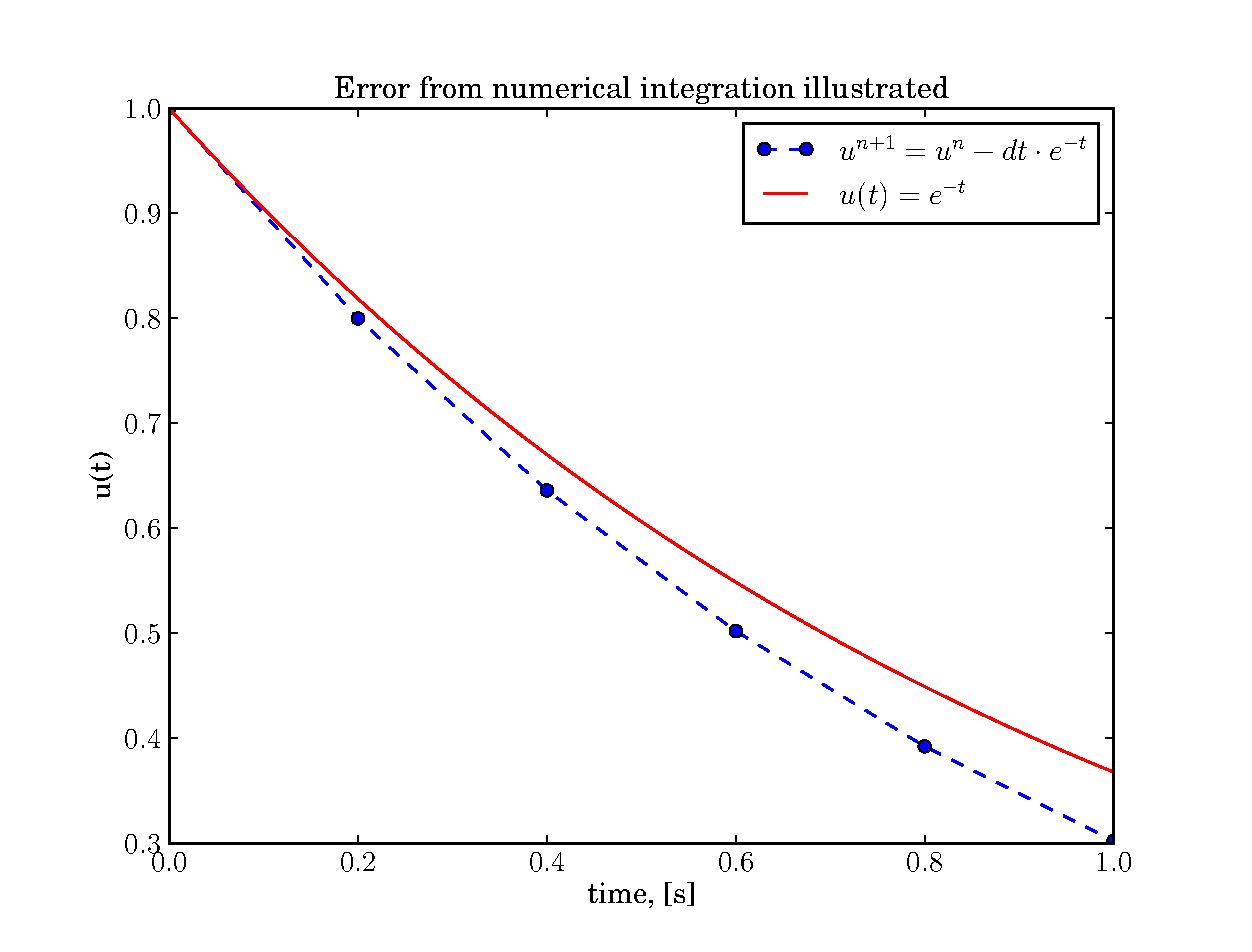
\includegraphics[scale=0.6]{Figures/numerical_error_illustrated.eps}
 \caption[Numerical errors illustration]{Illustration of how numerical errors appear. The dashed line shows the numerical solution of the equation $\frac{du}{dt} = -e^{-t}$ calculated with $6$ points using a FE scheme, while the full line is the exact solution $u(t)= e^{-t}$. The numerical scheme approximates the derivative as a constant between two points, an approximation which will become increasingly good as the resolution improves. }
 \label{illustrate_approximate_derivatives}
\end{figure}

% This can be done by choosing a solution to the PDE, doing a simulation which should yield the same solution and then comparing the two answers. 
% As argued in section \ref{} we will struggle with making the error from the random walk solver be much smaller than $\mathcal{O}(\Delta t)$. 
% We will therefore start by using a simple discretization of the PDE which also has a truncation error of $\mathcal{O}(\Delta t)$. 
% Figure \ref{errorplot_1d} shows the error norm (\ref{}) of only the PDE solver done in 1 dimension plotted for each timestep of the simulation. 
% The manufactured, exact solution is $u(x,t) = \exp\left(-\pi^2t\right)\cos(\pi x)$ and its initial condition is shown in figure \ref{}.

% \begin{figure}[H]
%  \centering
% %  \includegraphics[scale=0.7]{/home/fredriep/Dropbox/uio/thesis/doc/results/experiment_31102013_1017/results/initial_condition.eps}
%  \includegraphics[scale=0.7]{../doc/results/experiment_31102013_1017/results/initial_condition.eps}
%  \caption[Initial condition in 1d]{Initial condition of manufactured solution in 1d and the simulation.}
%  \label{initial_condition_1d}
% \end{figure}
% \begin{figure}[H]
%  \centering
% %  \includegraphics[scale=0.7]{/home/fredriep/Dropbox/uio/thesis/doc/results/experiment_31102013_1017/results/initial_condition.eps}
%  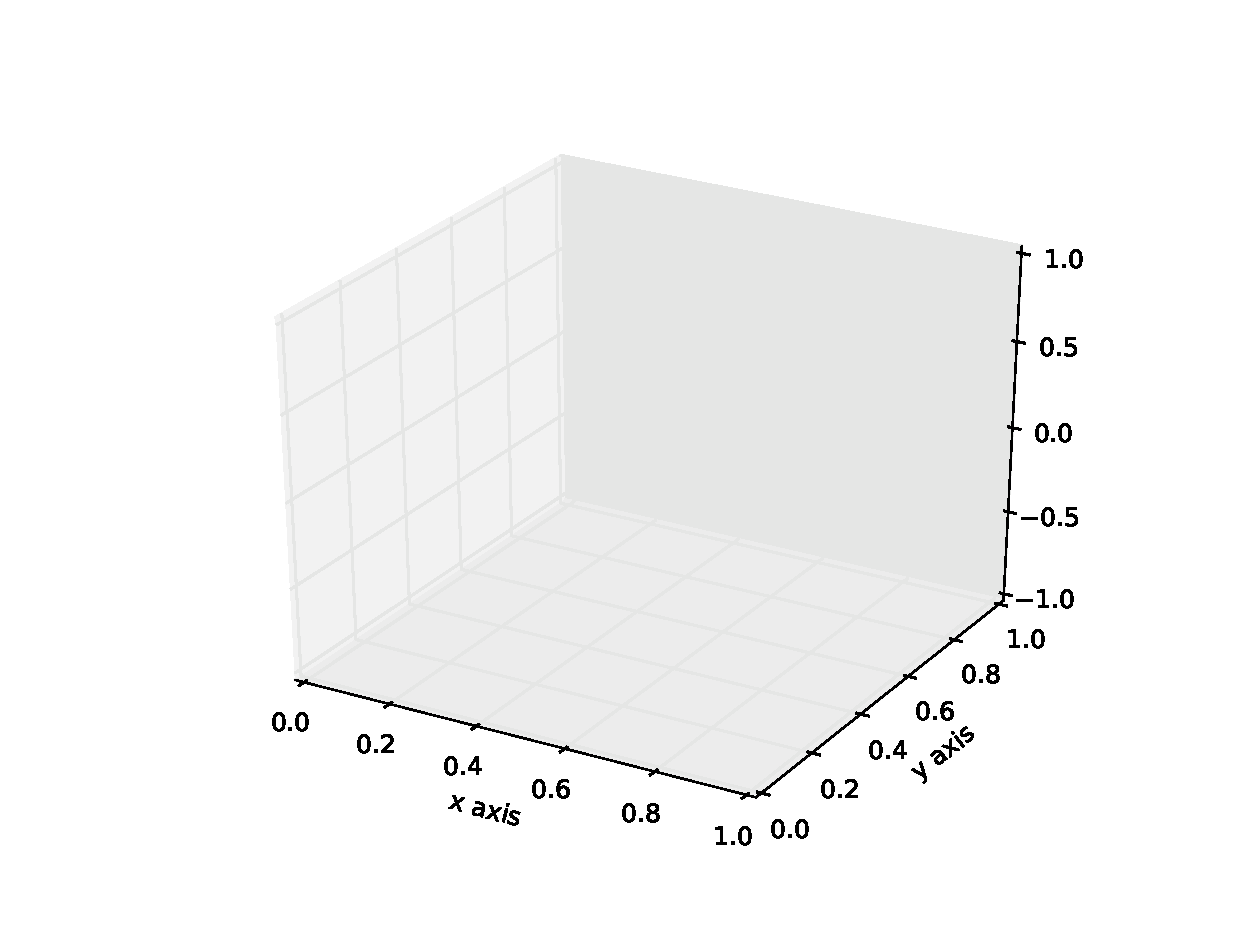
\includegraphics[scale=0.7]{Figures/InitialCondition2d.eps}
%  \caption[Initial condition in 2d]{Initial condition of manufactured solution in 2d and the simulation.}
%  \label{initial_condition_2d}
% \end{figure}
\section{Introduction}
\subsection{The error estimate}\label{error_estimate}
First and foremost the error measure, which will be denoted $\epsilon$ will be specified.
Throughout this thesis the term error is used quite lazily, but unless something else is specified we refer to the expression 
\begin{equation}
 \epsilon(t_i) = ||u_e(t_i)-u(t_i)||_2
\end{equation}
where $u_e$ is an exact (manufactured) solution to the equation, and $u$ is the result from the numerical simulation. 
This error-estimate is used because it is time-dependent, thus explicitly showing how the error evolves over time. 
The error is calculated over the entire mesh, which will clearly show if the error from the random-walk areas are dominating, or (otherwise) how the PDE-scheme is holding up.
Another error estimate that will be used later is the integrated norm of the previously mentioned error estimate. 
This will be used for the convergence tests to make sure that no effects of simulating for a long time are overlooked, and is defined as 
\begin{equation}
 \epsilon = \sqrt{\sum\limits_i h^2\epsilon(t_i)}
\end{equation}
where $h$ is the parameter in question (usually $\Delta t$).

\subsection{Verification techniques}
There are quite a few ways to verify an implementation. This thesis will focus on three which are considered adequate for no particular reason. 
Unfortunately some of the tests require isolating one error-term, meaning that the test works better if the stability criterion for the FE scheme is broken. 
The result of this is that some of the tests are only done on the BE scheme. 
Fortunately, the BE scheme will be used for the actual simulations and will see more thorough verification.

\begin{itemize}
 \item Method of manufactured solutions\\
 A normal way of checking that our scheme of choice is implemented correctly is by constructing an exact solution to the equation and checking that the error is of the expected order. 
Since the software contains both an explicit FE scheme and an implicit BE scheme they will both be verified alongside one another. 
We will start with the simplest diffusion equation (eq. \eqref{simple_diffusion_equation}) and add complexity until the expression verifies all parts of the implementation. 
Both schemes are expected to have an error-term of the order of $\Delta t$, which in the FE case is limited by a stability criterion. 
Next, the initial condition for a simulation is set to the exact solution at $t=0$, and the simulation can be run with different parameter values. 
This approach makes it trivial to calculate the error, seeing as the solution is known, and to check that it takes the expected values.\\
There are some variations of this method which should be mentioned. 
Setting the manufactured solution to a constant (or a linear polynomial if the boundary conditions allow it) should eliminate the error completely since the derivative is zero which eliminates the numerical error. 
This is also a nice way of verifying that the scheme conserves energy (or matter for that matter).

\item Exact numerical solutions\\
For the explicit schemes, exact solutions to the scheme itself can be found seeing as the scheme is a difference equation. The calculations are shown step-by-step in section \ref{exact_numerical_solution}.
\item Convergence tests\\
This must be combined with the manufactured solution, but takes a slightly different approach to quantifying the error estimate. We start by calculating some form of error estimate, and chose a value to represent the error of the entire simulation. This could be the maximum error for the entire simulation, or an integrated measure. 
Multiple simulations will be done while improving the parameter of interest, for example how the size of the time-step influences the error. 
Finally, a number indicating the improvement in the error estimate by improving the parameter in question is calculated. 
This number indicates the order of convergence which is one for FE and BE since the error goes as $\mathcal{O}(\Delta t)$, and two for our approximation to the second derivative in space since the error goes as $\mathcal O(\Delta x^2)$.
A convergence rate of 1 means that halving the parameter will (roughly) halve the error, while the same reduction for a second order convergence will reduce the error by 4.
\end{itemize}


\section{Verification of PDE solvers}
To verify the implementation of the PDE-solvers, the steps outlined in the previous section will now be performed. 
The approach will be to begin the testing on the simplest diffusion equation using the full implementation, and add complexity along the way. 
This is another way of verifying that the implementation is correct since the average of the anisotropic diffusion coefficient at two mesh-points is the same as the diffusion constant if there is no change over the mesh-points. Effectively this is the same as having only a constant. 
The same applies to setting the drift-velocity equal to zero. 

Since both the FE and BE discretization have been implemented both of them will be tested, but for the most part the BE discretization will be used in simulations because of its unconditional stability.
For most of the tests the exact (manufactured) solution will be equation \eqref{manufactured_solution_2D} which satisfies the diffusion equation if the diffusion constant is 1 and $x\in[0,1]$. 
In 1D the solution will be correct since $y=0$ over the entire mesh. 
\begin{equation}\label{manufactured_solution_2D}
 e^{-\pi^2t}\cos(\pi x)\cos(\pi y) +1
\end{equation}


All of the verification on the PDEs will be done without adding random walkers. The implementation of these will be done individually, along with some tests of the combined solver in the end.

\subsection{Manufactured Solutions}

As mentioned the solution
\begin{equation}\label{manifactured_solution_1D}
 u(x,t) = e^{-t\pi^2}\cos(\pi x) +1
\end{equation}
is chosen because it fulfills the chosen boundary conditions.
Equations \eqref{manufactured_prof_pt1} and \eqref{manufactured_prof_pt2} prove that the manufactured solution does indeed fulfill the diffusion equation (eq. \ref{simple_diffusion_equation}).
\begin{align}
 \frac{\d }{\d t}e^{-t\pi^2}\cos(\pi x) +1 &= D\frac{\d^2}{\d x^2}e^{-t\pi^2}\cos(\pi x) +1\label{manufactured_prof_pt1}\\
 -\pi^2e^{-t\pi^2}\cos(\pi x) &= -\pi^2e^{-t\pi^2}\cos(\pi x) +1 \label{manufactured_prof_pt2}\\
 \implies 1 &= 1 \nonumber
\end{align}

The error in space is determined by two factors, the actual error caused by the approximation to the second derivative, which is of the order of $\Delta x^2$ and, in the FE case, the error term coming from the time derivative due to the stability criterion (eq. \ref{stability}), which is also of the order $\Delta x^2$. \\
Figure \ref{verification_FE1D} shows error and convergence plots for the FE scheme in 1D. 
For longer simulations, the analytic solution is expected to reach a steady state which is found in the limit of large $t$, 

\begin{equation}
 u(x,t\to\infty) \to e^{-\infty}\cos(\pi x) +1 \to 1
\end{equation}
The numerical scheme should be able to represent this to machine precision ($10^{-16}$), meaning that the numerical solution should start converging to zero after some number of times steps, but this might depend on how the derivatives as estimated so we say that it should in the very least stabilize. 
The error plots in Figure \ref{verification_FE1D:errorplot} clearly show that the error tends to zero as the steady state is reached. 
As for the convergence, it is not perfect, but it could have been worse. There might be some effects from the spatial error which influences the error, but due to the stability criterion the time step cannot be increased beyond $\frac{\Delta x^2}{2}$ which prevents isolating the error from the time derivative. 
Considering the tests which will be done later with respect to the numerical exact, the scheme seems to be performing fairly good, if not perfect.

\begin{figure}[H]
\centering
\begin{subfigure}[b]{0.48\textwidth}
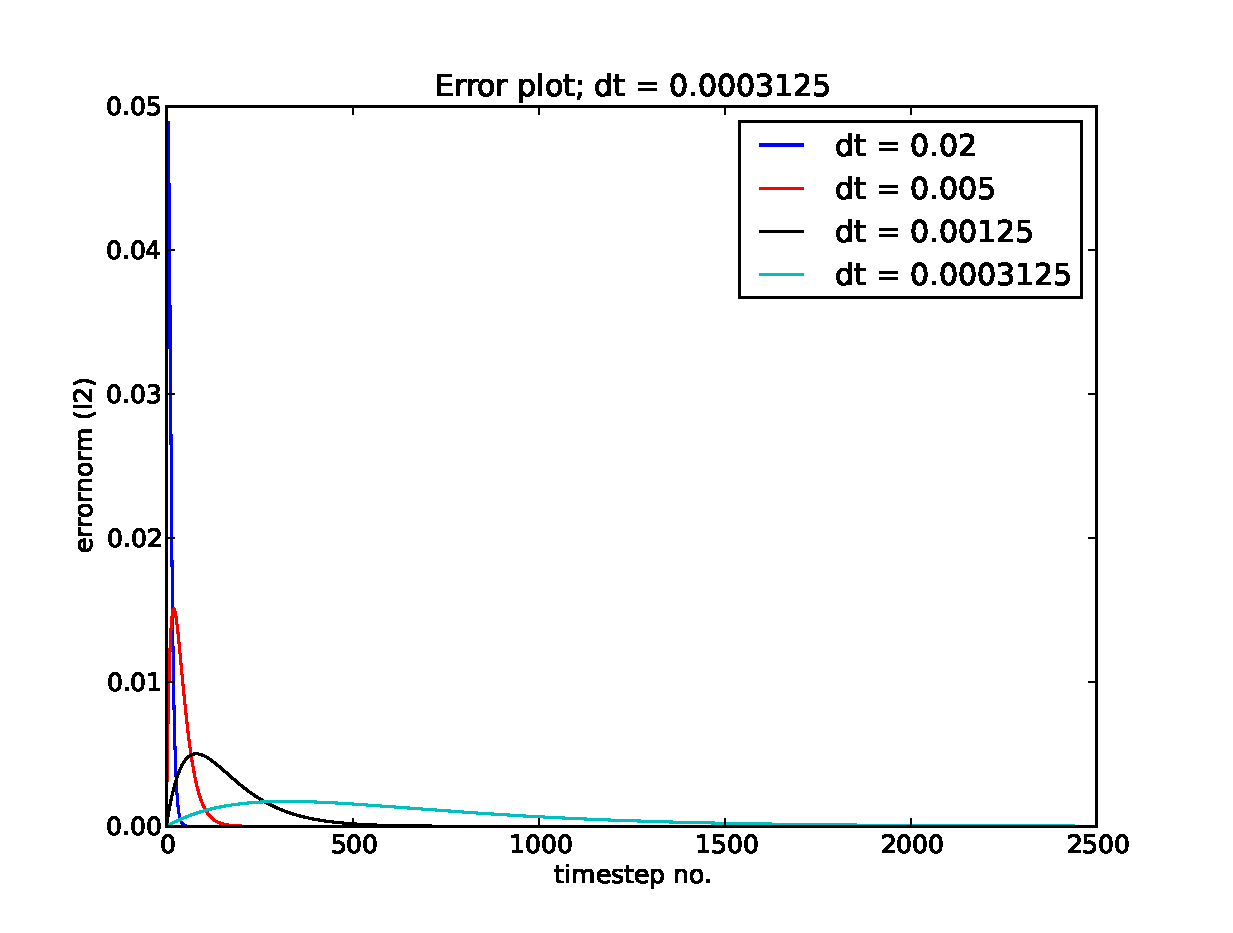
\includegraphics[width=\textwidth]{../doc/results/experiment_18042014_1014_convergencetest_FE1D/results/errorplot.eps}
\caption{}% Replace this figure with a convergence rate plot for the FE discretization.
\label{verification_FE1D:errorplot}
\end{subfigure}
\begin{subfigure}[b]{0.48\textwidth}
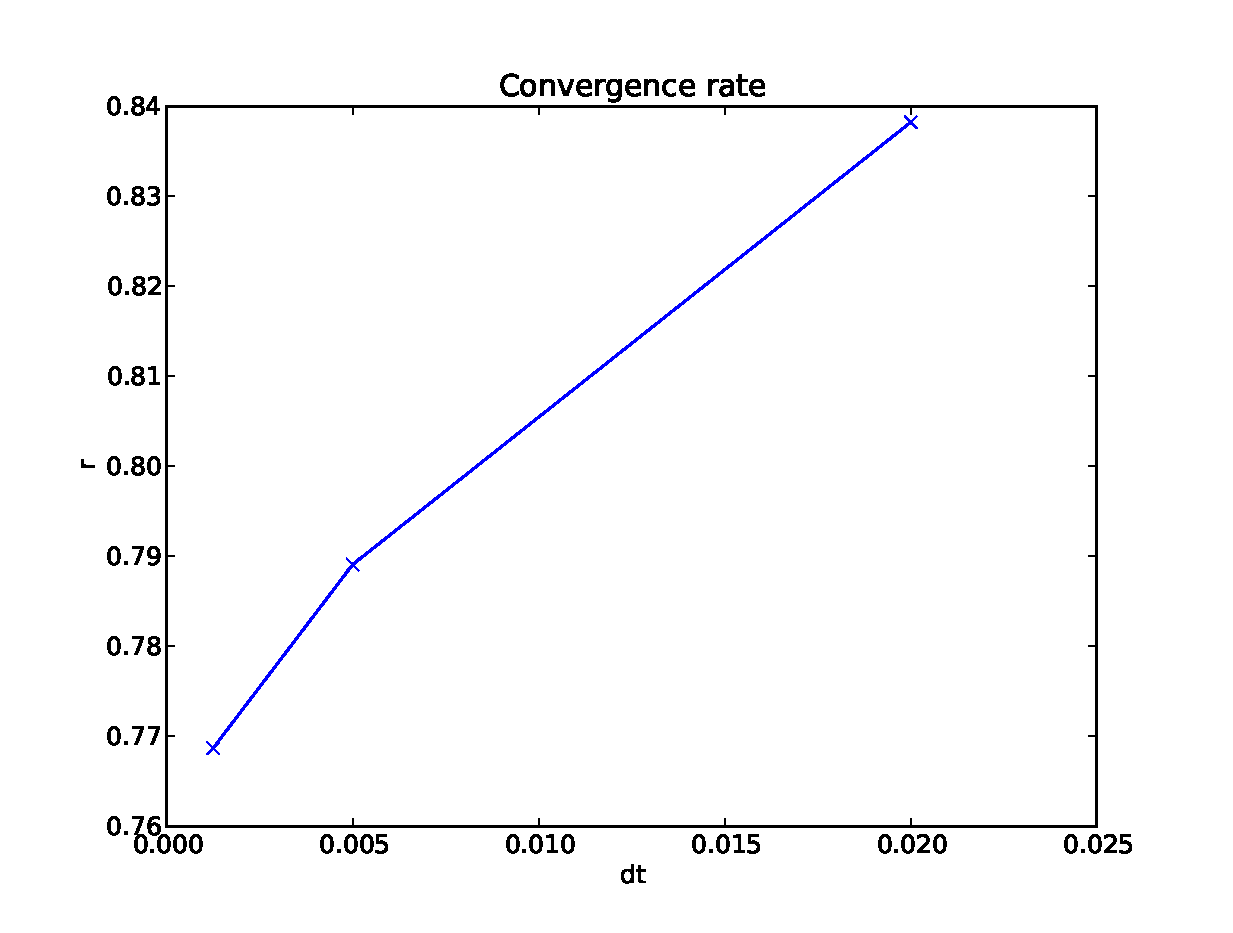
\includegraphics[width=\textwidth]{../doc/results/experiment_18042014_1014_convergencetest_FE1D/results/ConvergenceTest.eps}
 \caption{}
 \label{verification_FE1D:convergence}
\end{subfigure}
\caption[Error plot for 1D Forward Euler scheme]{Numerical error for 1D Forward Euler discretization of the PDE. Nothing else is done to the simulation.}
\label{verification_FE1D}
\end{figure}

Testing of more advanced implementations requires some additional calculations in order to still have the same manufactured solution as before. 
The variable diffusion coefficient 
$$D(x) = \pi x$$
is introduced and the drift term is still zero. 
The new source term required is 

\begin{align*}
 -\pi^2\exp\left(-\pi^2t\right)\cos\left(\pi x\right) &= -\pi\exp\left(-\pi^2t\right)\frac{\d}{\d x}\pi x\sin(\pi x) +f(x,t) \\
 -\pi^2\cos\left(\pi x\right) &= -\pi^2\left(\sin(\pi x) + \pi x\cos(\pi x)\right) +\tilde{f}(x) \\
 \tilde{f}(x) &= \pi^2\left(\sin(\pi x) +\cos(\pi x)(\pi x-1)\right)
\end{align*}
where $f(x,t) = \exp\left(-\pi^2t\right)\tilde{f}(x)$. Figure \ref{anisotropic_diffusion_verification} shows the error norm of the result of simulations of this equation with different values of $\Delta t$.

\begin{figure}[H]
\centering
\begin{subfigure}[b]{0.48\textwidth}
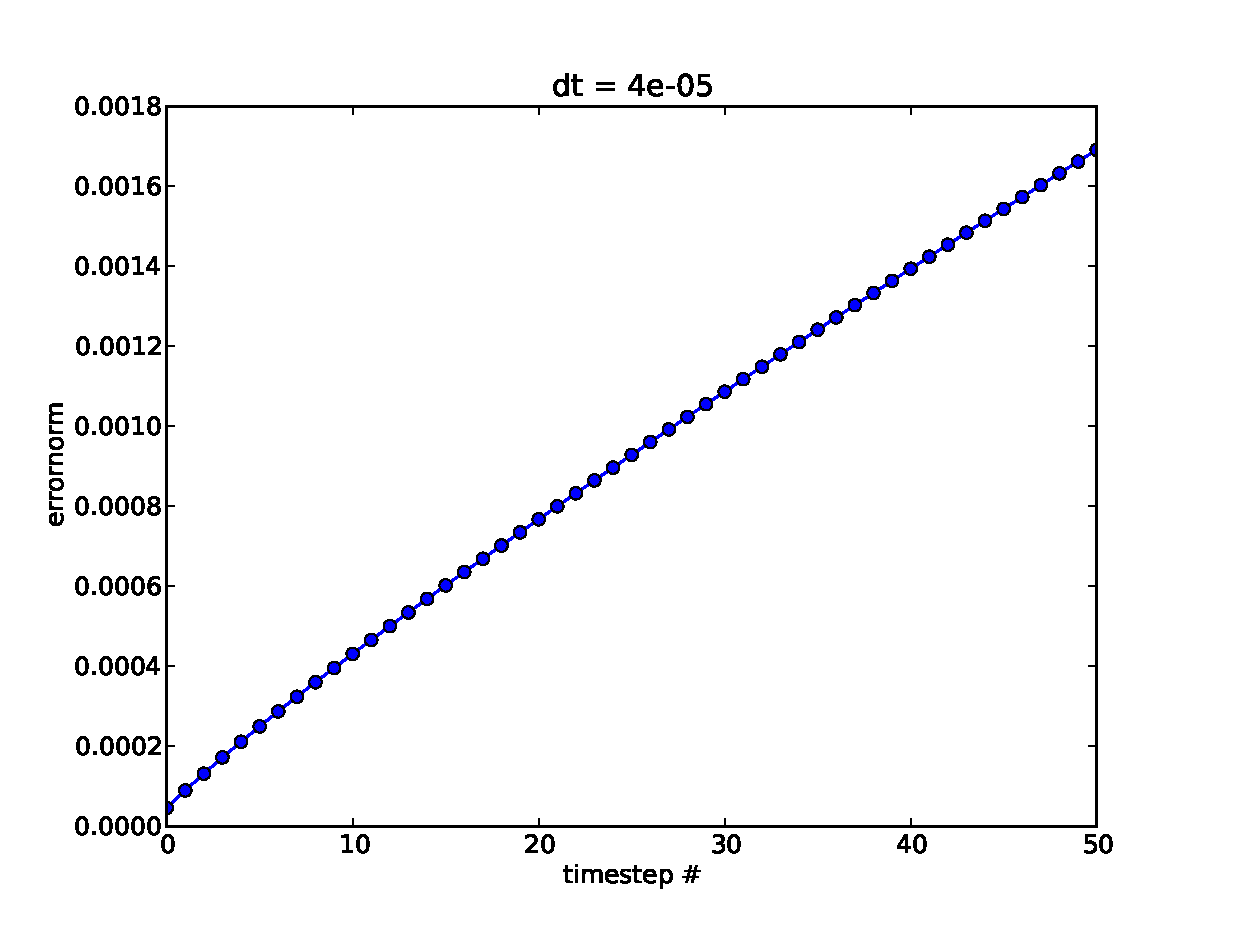
\includegraphics[width=\textwidth]{../doc/results/experiment_05112013_1303/results/deterministic_errorplot.eps}
\caption{}
\label{anisotropic_diffusion_verification:single_dt}
\end{subfigure}
\begin{subfigure}[b]{0.48\textwidth}
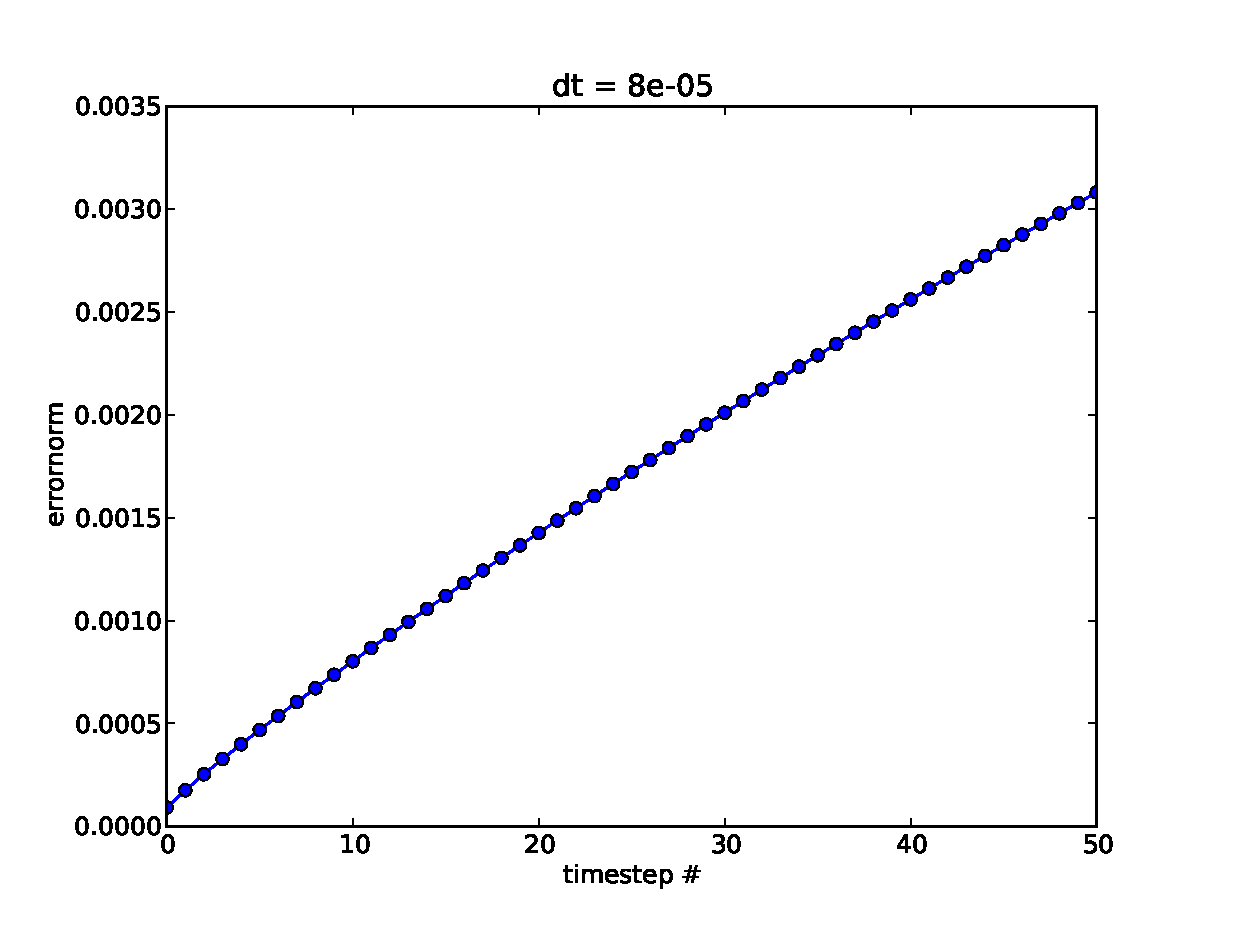
\includegraphics[width=\textwidth]{../doc/results/experiment_05112013_1304/results/deterministic_errorplot.eps}
\caption{}
\label{anisotropic_diffusion_verification:double_dt}
\end{subfigure}
\caption[Verification of anisotropic diffusion equation implementation]{Verification of anisotropic diffusion equation implementation}
\label{anisotropic_diffusion_verification}
\end{figure}
Again, the error is of the order of $\Delta t$ and is roughly halved by halving $\Delta t$.

\subsection{Convergence Tests}


The next step in testing the implementation will be to perform a convergence test in time. 
The spatial convergence test is toned down because an incorrect implementation of the spatial derivative would be clearly visible both in the visualization of the simulation (the solution blows up), and in the error plot seeing as the spatial error would dominate.
As mentioned, the convergence tests are carried out by doing several simulations with different values for $\Delta t$ and comparing the errors by equation \ref{convergence_rate_def}. 
\begin{equation}\label{convergence_rate_def}
 r = \frac{\ln(E_{i+1}/E_i)}{\ln(\Delta t_{i+1}/\Delta t_i)}
\end{equation}
A result of such an experiment for the FE scheme using the $\Delta t$ values listed below is found in Figure \ref{convergence_test:FE}. 
The expected value of r is approximately 1. The result is not perfect, but still close to 1. 
For the BE scheme we get the convergence rate shown in Figure \ref{convergence_test:BE}. Again, the expected order of convergence is 1 and this time the result is almost perfect.


% \begin{lstlisting}
%  dt = [1e-4,1e-5,1e-6,1e-7,1e-8]
% \end{lstlisting}

\begin{figure}[H]
 \centering
 \begin{subfigure}[t]{0.48\textwidth}
 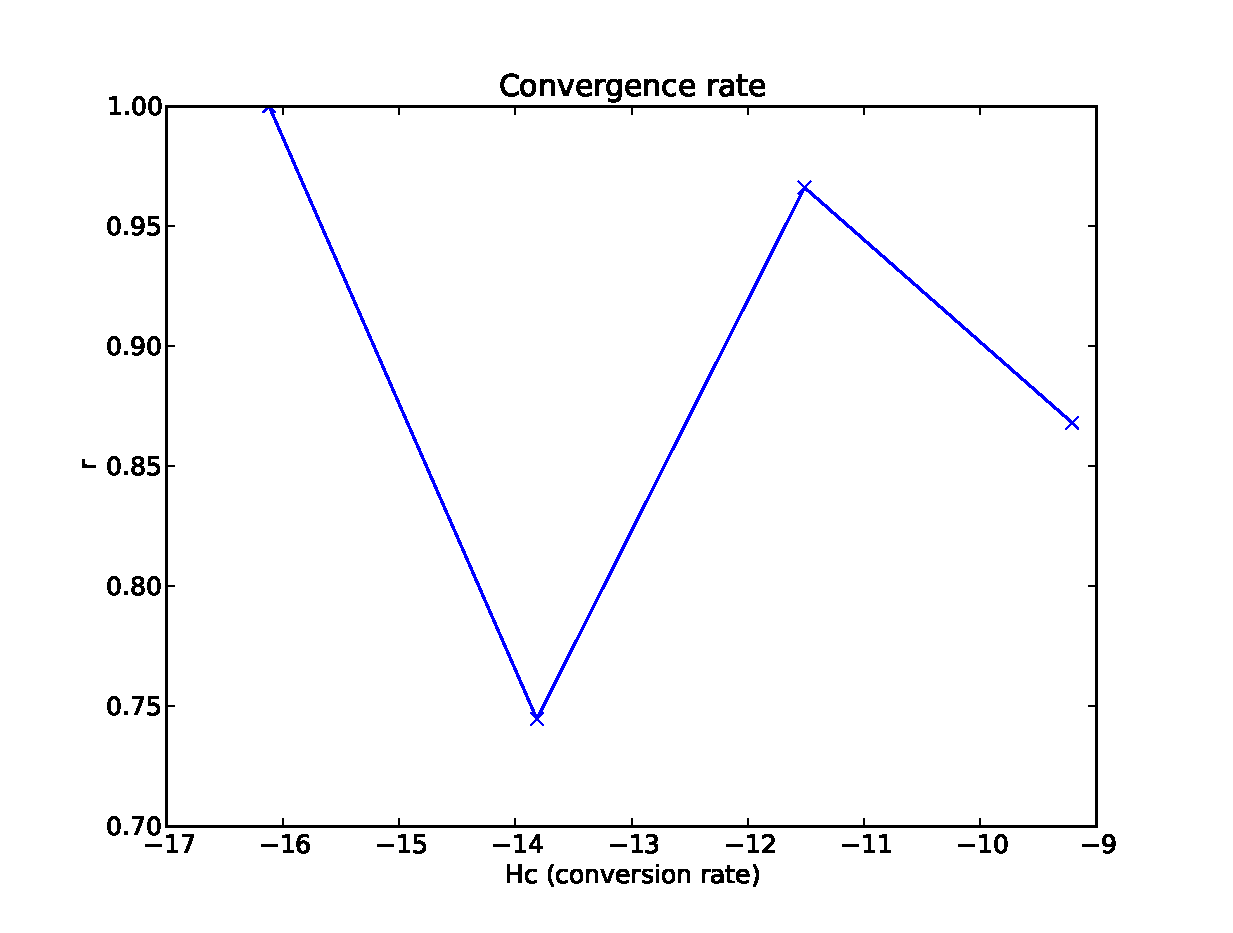
\includegraphics[width=\textwidth]{../doc/results/experiment_27112013_1017/results/ConvergenceTest.eps}
 \caption{Convergence test for the FE scheme. The x axis is $\ln(\Delta t)$.}
 \label{convergence_test:FE}
\end{subfigure}
\begin{subfigure}[t]{0.48\textwidth}
 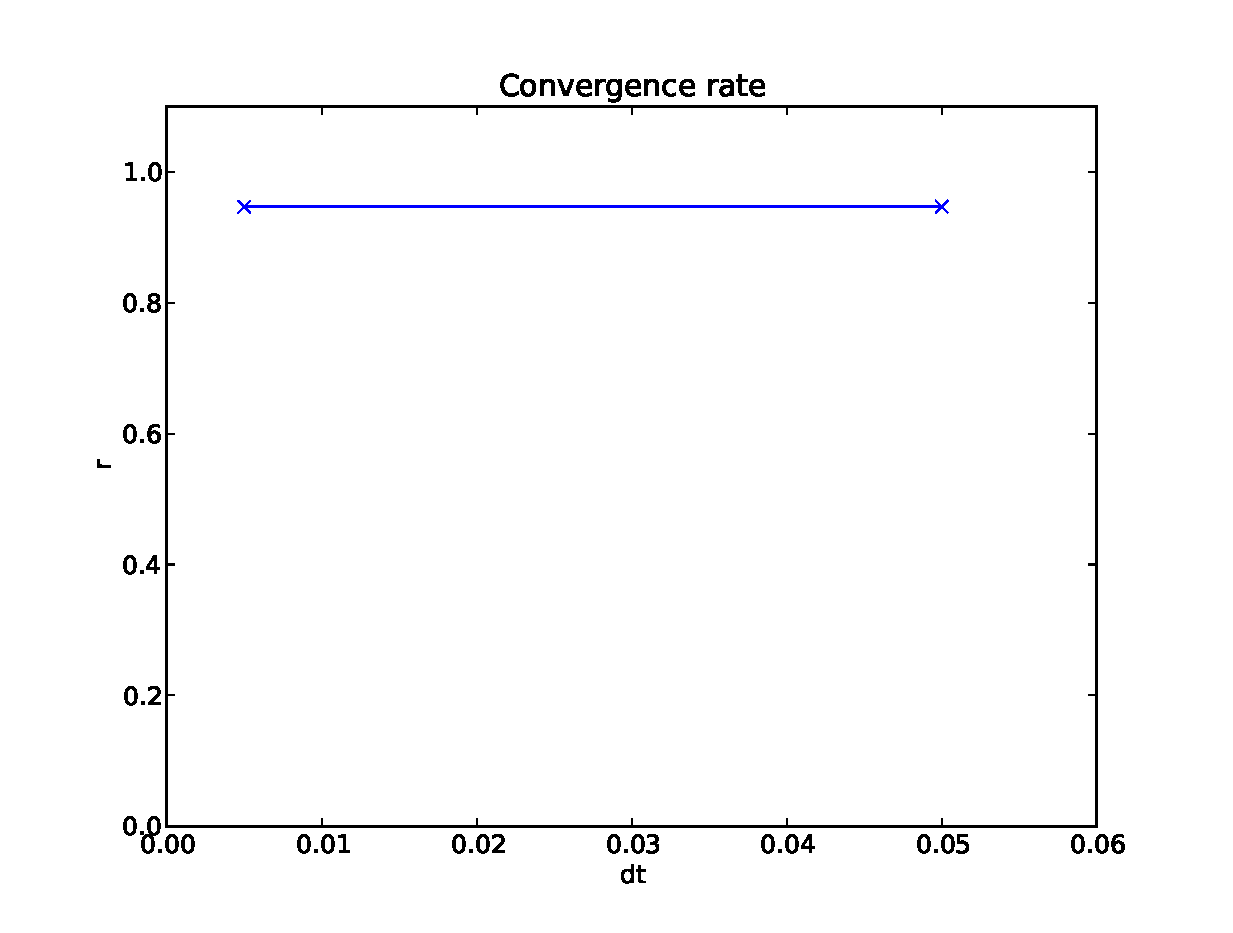
\includegraphics[width=\textwidth]{../doc/results/experiment_18042014_1450_convergencetest_BE2D/results/ConvergenceTest.eps}
 %remove folders : [experiment_13012014_0925_Simple1DConvergenceTestBE]
 \caption{Convergence test for the BE scheme.}
 \label{convergence_test:BE}
\end{subfigure}
\caption[Convergence tests in 1D]{Convergence tests for explicit and implicit schemes solving the simple diffusion equation (eq. \eqref{simple_diffusion_equation}).}
\label{convergence_test}
\end{figure}

We can also do a convergence test, equal to the one we did in 1D, to check that the scheme converges to 1 (by equation \eqref{convergence_rate_def}) for smaller $\Delta t$ in 2D as well. 
The results of this test are shown in Figure \ref{convergence_test_FE_2d} and it does converge nicely to one.

\begin{figure}[H]
\centering
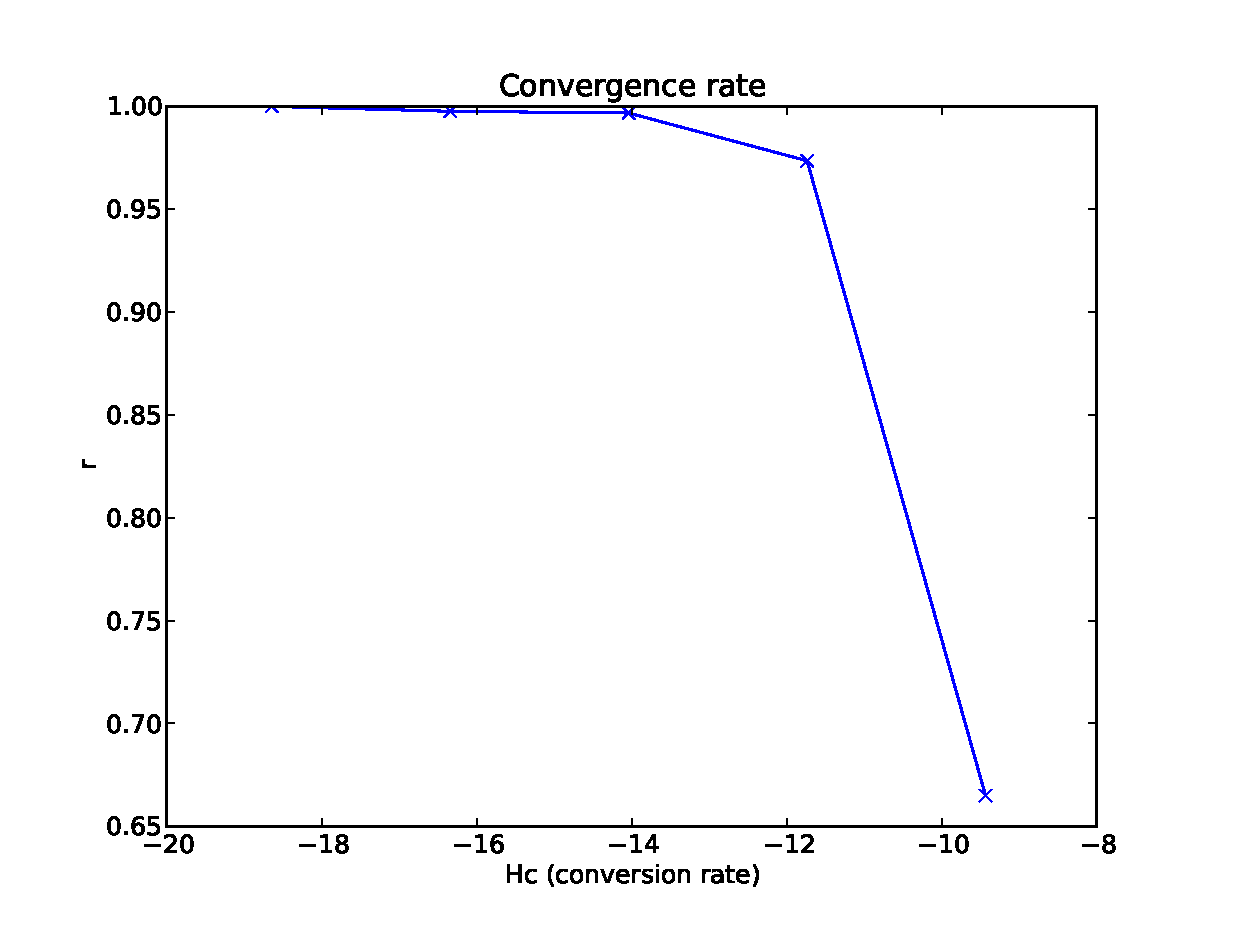
\includegraphics[scale=0.5]{../doc/results/experiment_29112013_1709/results/ConvergenceTest.eps}
\caption[Convergence test FE 2D]{Convergence test for the FE scheme in 2D using $\Delta t$ ranging from the stability criterion $\frac{\Delta x\Delta y}{5}$ to the same ratio divided by 100000 in increments of $10^{-1}$.}
\label{convergence_test_FE_2d}
\end{figure}

\subsubsection{Spatial convergence}

Figure \ref{spatial_convergence_test} shows the converge for the spatial error. 
This test is done only using the implicit scheme since it is an advantage for the spatial error, which is of second order, to be larger than the error from the time discretization. 
Because of the stability criterion for the FE scheme it will break down for these tests, and not give the desired results. 
Another complicating factor is having the time step sufficiently smaller than the spatial resolution. 
As Figure \ref{spatial_convergence_test} shows, the test was not perfect, however it starts out with a convergence of almost 2 done on a coarser mesh. 
The normal error plot is also included in the figure to illustrate that the improvement is significant. 

\begin{figure}[H]
 \centering
 \begin{subfigure}[b]{0.48\textwidth}
  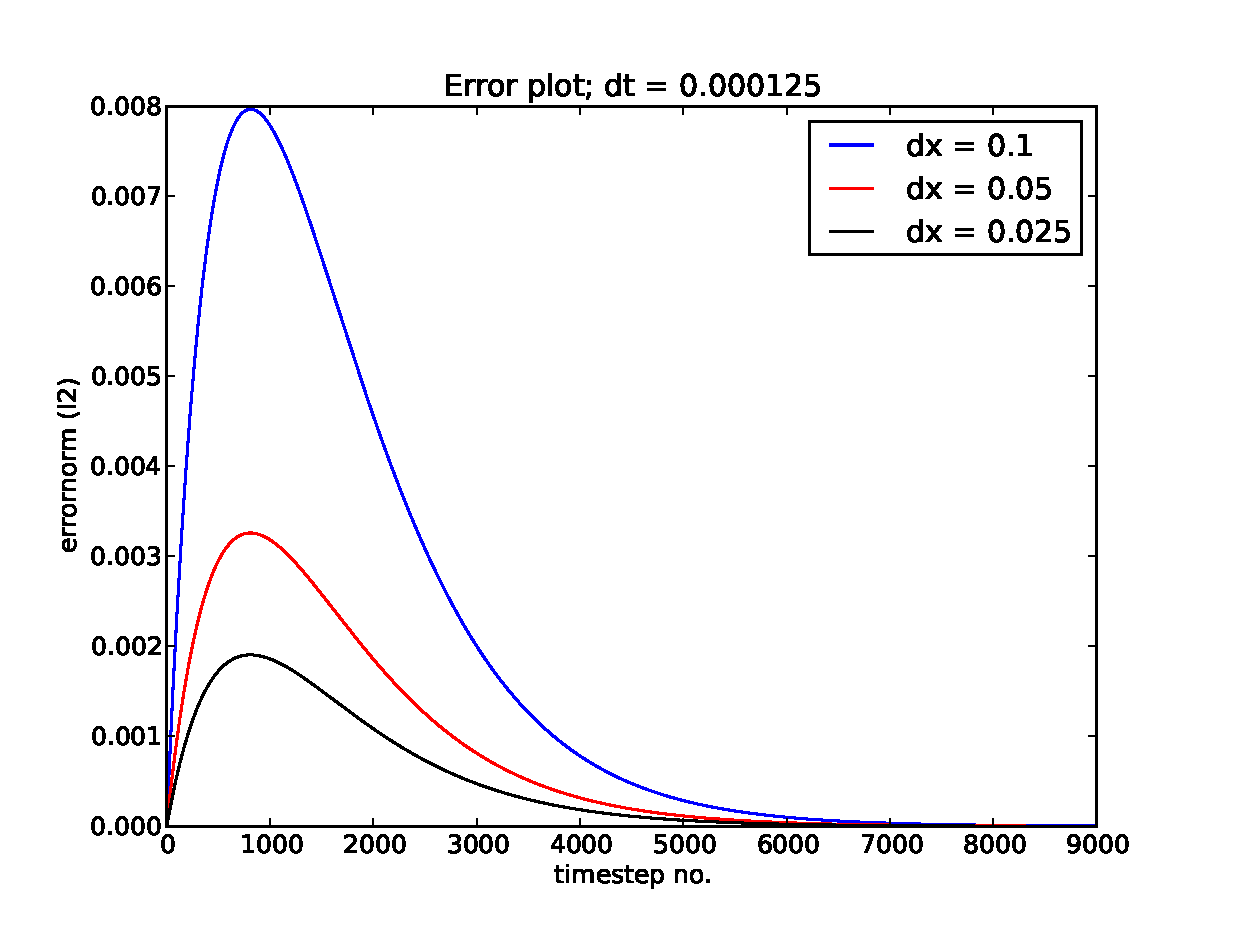
\includegraphics[width=\textwidth]{../doc/results/experiment_14042014_1303_convergence_tests_etc/results/errorplot.eps}
  \caption{Error plot}
 \end{subfigure}
 \begin{subfigure}[b]{0.48\textwidth}
  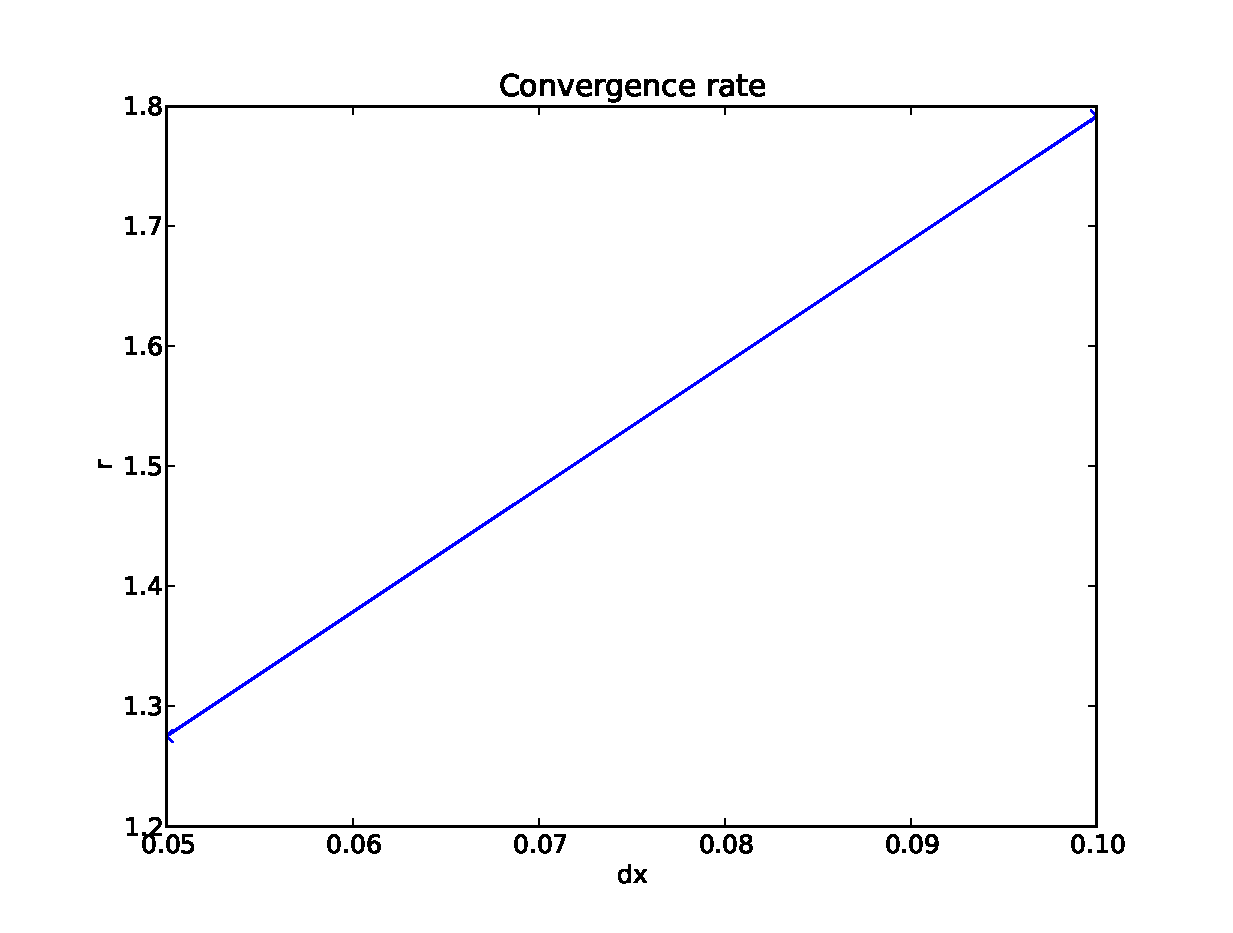
\includegraphics[width=\textwidth]{../doc/results/experiment_14042014_1303_convergence_tests_etc/results/ConvergenceTest.eps}
  \caption{Convergence test}
 \end{subfigure}
 \caption[Verification of spatial derivative]{Error plot (a) and convergence test (b) focusing on the spatial error term. This test requires the time step to be much smaller than $\Delta x^2$ in order for the spatial error to dominate. As is apparent from figure b, the convergence test is difficult to get right. Notice, however that the first value in the convergence test is close to 2, and that the second one is clearly larger than 1 suggesting that other effects might be at play. The test was done in 1D using the BE discretization with $\Delta t = \frac{1}{8000}$ for all values of $\Delta x$. This value is problematic because it is only a factor $\frac{1}{5}$ smaller than $\Delta x^2$ for $\Delta x = \frac{1}{40}$ which is the last simulation.}
 \label{spatial_convergence_test}
\end{figure}


\subsection{Exact numerical solution}\label{exact_numerical_solution}

Both schemes can be reformulated as difference equations, and will therefore have some form of exact solution. 
Comparing a simulation to the expected exact numerical solution is a good way to verify that the implementation does what it is expected to do. 
The numerical exacts are expected to be represented to more or less machine precision, though some deviances might occur.

As was done in section \ref{some_words_on_PDEs}, the schemes must first be reformulated as a theta-rule discretization
\begin{equation}\label{theta_rule_difference_equation}
  \frac{u^{n+1}-u^n}{\Delta t} =\theta D\Delta t u_{xx}^{n+1} +(1-\theta)D\Delta t u_{xx}^n
\end{equation}

where $u_{xx}^n$ denotes the double derivative of $u$ at time step $t^n$.

\subsubsection{The FE scheme}

Inserting $\theta=0$ in equation \eqref{theta_rule_difference_equation} yields the FE scheme. The first few iterations are written out as

\begin{align*}
 u^1 &= D\Delta t u_{xx}^0 + u^0 \\
 u^2 &= D\Delta t u_{xx}^1 + u^1 = D\Delta t\left[D\Delta t u_{4x}^0 + u_{2x}^0\right] + u^0\\
 &= \left(D\Delta t\right)^2 u_{4x}^0 + 2D\Delta t u_{2x}^0+ u^0 \\
 u^3 &= D\Delta t u_{xx}^2 + u^2 = D\Delta t\left[\left(D\Delta t\right)^2 u_{6x}^0 + 2D\Delta t u_{4x}^0+ u_{2x}^0\right] + \left(D\Delta t\right)^2 u_{4x}^0 + 2D\Delta t u_{2x}^0+ u^0\\
 &= \left(D\Delta t\right)^3 u_{6x}^0 + 3\left(D\Delta t\right)^2 u_{4x}^0+ 3D\Delta tu_{2x}^0 + u^0 \\
 u^4 &= D\Delta t u_{xx}^3 + u^3 = \dots \\
 &= \left(D\Delta t\right)^4 u_{8x}^0 + 4\left(D\Delta t\right)^3 u_{6x}^0+ 6\left(D\Delta t\right)^2 u_{4x}^0 + 4D\Delta t u_{2x}^0 + u^0 
\end{align*}

This can be generalized to 
\begin{equation}
 u^{n+1} = \sum\limits_{i=0}^n {n\choose i}\left(D\Delta t\right)^iu^0_{2ix}
\end{equation}

where the initial condition is known from equation \eqref{manifactured_solution_1D}
\begin{equation*}
 u^0_{2ix} = \left(-1\right)^i\pi^{2i}\cos(\pi x)
\end{equation*}

Inserting the initial condition results in the exact solution to the FE scheme
\begin{equation}
 u^{n+1} = \sum\limits_{i=0}^n {n\choose i}\pi^{2i}\left(-1\right)^i\left(D\Delta t\right)^i\cos(\pi x)
\end{equation}

Notice that the analytical spatial derivative has been used rather than the approximation to the spatial derivative. 
In the same way as for the time derivative, the approximation to the spatial derivative must be inserted. 
\begin{align*}
 u^0_{xx} &= \frac{1}{\Delta x^2}\left(\cos(\pi(x+\Delta x)) -2\cos(\pi x) +\cos(\pi(x-\Delta x))\right) \\
 &= \frac{2}{\Delta x^2}\left(\cos(\pi\Delta x)-1\right)\cos(\pi x)\\
 u^0_{4x} &= [u^0_{xx}]_{xx} \frac{1}{\Delta x^2}\left[\frac{u^0_{xx}}{\cos(\pi x)}\left(\cos(\pi(x+\Delta x)) -2\cos(\pi x) +\cos(\pi(x-\Delta x))\right)\right]\\
 &= \frac{4}{\Delta x^2}\left(\cos(\pi\Delta x)-1\right)^2\cos(\pi x)\\
 &\dots
\end{align*}

% u^0_{4x} &= [u^0_{xx}]_{xx} \frac{1}{\Delta x^2}\left[\frac{2}{\Delta x^2}\left(\cos(\pi\Delta x)-1\right)\left(\cos(\pi(x+\Delta x)) -2\cos(\pi x) +\cos(\pi(x-\Delta x))\right)\right]\\

This pattern continues, and the exact numerical solution can be expressed by equation \eqref{numerical_solution} in 1D for the previously mentioned initial condition.
\begin{equation}\label{numerical_solution}
  u^{n+1} = \sum\limits_{i=0}^n {n\choose i}\left(D\Delta t\right)^i\frac{2^i}{\Delta x^{2i}}\left(\cos(\pi\Delta x)-1\right)^i\cos(\pi x)
\end{equation}

The FE scheme is expected to represent this solution more or less to machine precision, at least to $15$ digits. 
There are, however two issues with the solution \eqref{numerical_solution}:
\begin{itemize}
 \item $\Delta x^{2i}$ will quickly tend to zero, and the computer will interpret it as zero. This will cause division by zero, which again results in ``Not a number'' (nan) and ruins the simulation. This can be fixed rather simply by testing if $\Delta x^{2i}>0$ and returning zero if the test returns false.
 \item ${n\choose i}$ goes to infinity for large n and i. The computer can only represent numbers up to $\sim10^{308}$, which limits the number of steps to $170$ since $n!>10^{308}$ for $n>170$. 
 The argumentation for dropping the troublesome terms is given below.
%  Figure \ref{convergence_exact_numerical_1d_n145} shows that at least for relatively few time steps the troublesome terms can be dropped, but effectively this limits the simulation to some 170 steps regardless of the value of $\Delta t$.
\end{itemize}

As a side note, equation \eqref{numerical_solution} illustrates how the stability criterion (eq. \ref{stability}) comes into place. 
The solution used in the derivation of the stability criterion assumes an amplification factor $A^n$ to replace the exponential amplification in the actual solution. 
This amplification factor can be found in equation \eqref{numerical_solution} as 
$$\left(\frac{2D\Delta t}{\Delta x^2}\right)^i$$
Inserting a time step larger than the stability criterion ($\Delta t \leq \frac{\Delta x^2}{2D}$) will make the amplification factor $A$ larger than one which in turn will make the solution blow up.
This also illustrates why the terms where 
$$ \frac{1}{\Delta x^{2i}} \to \infty$$
 can be dropped. 
 By the stability criterion, the time step will cancel out $\Delta x^2$, and the result will be some number smaller than 1 raised to a rather large power, $i$, resulting in something comparable to zero.\\
% 
% \begin{figure}[H]
%  \centering
%  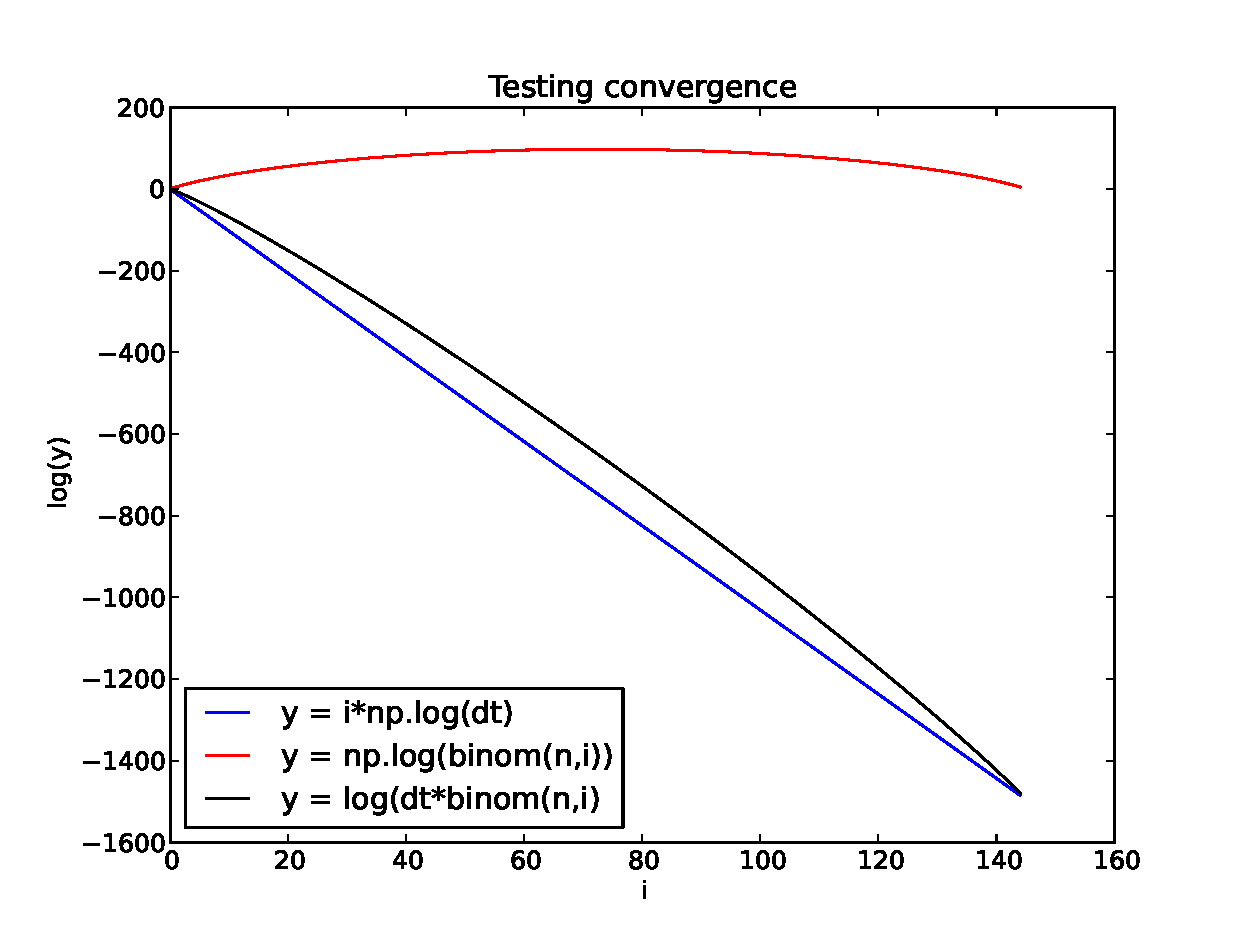
\includegraphics[scale=0.5]{Figures/convergence_exact_numerical_1d_n145}
%  \caption{Testing the relation between $\left(D\Delta t\right)^i$ and the binomial coefficients.}
%  \label{convergence_exact_numerical_1d_n145}
% \end{figure}

The results from testing the FE scheme are found in Figure \ref{errorplot_numerical_exact_FE_1D}. We see that the error in the worst case is about an order of magnitude worse than expected. This is most likely due to the fact that we are cutting part of the solution, and over several time steps the error we do might accumulate.
This is most likely a 

\begin{figure}[H]
 \centering
 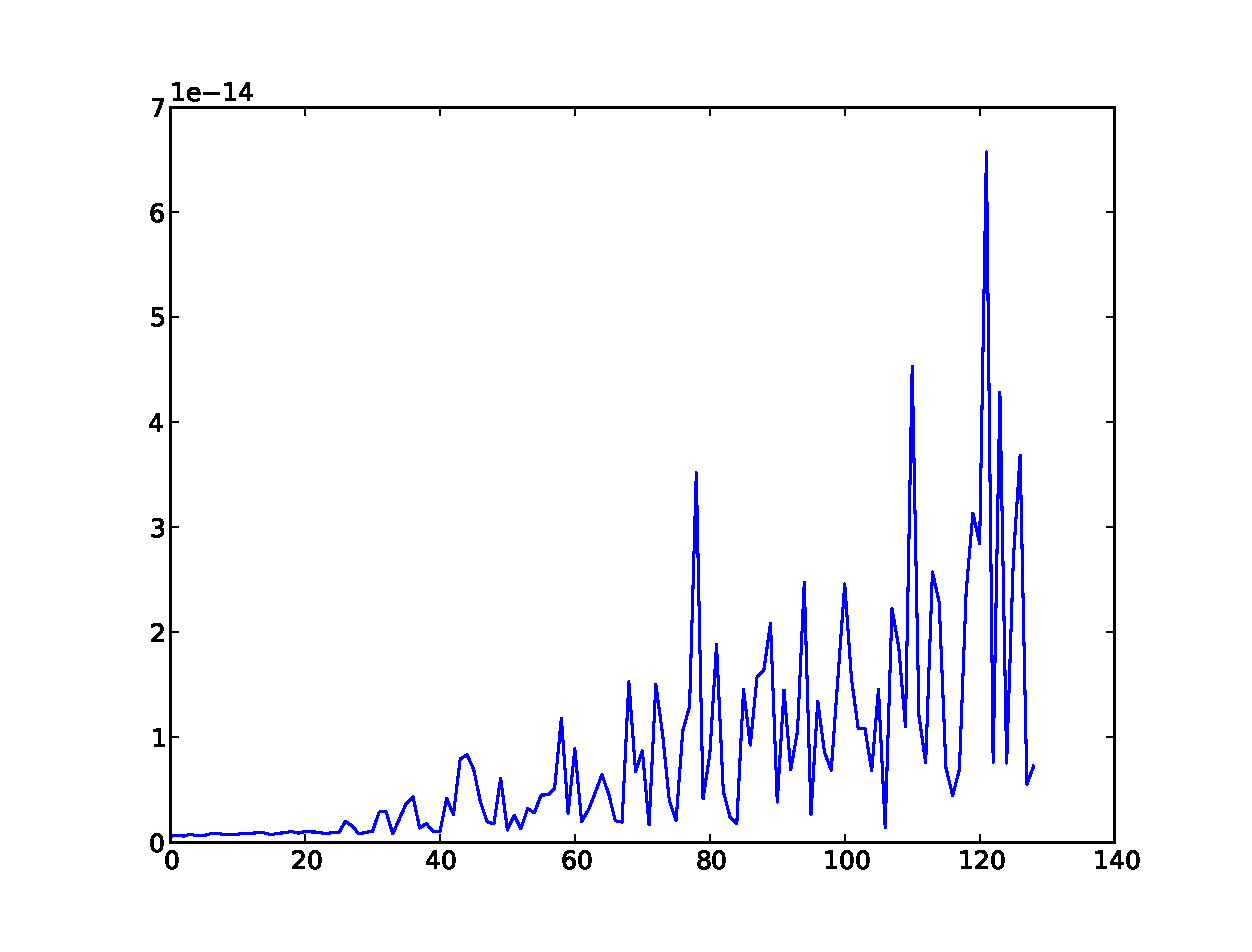
\includegraphics[scale=0.7]{Figures/exact_numerical_1d_n130.eps}
 \caption[Verification for exact numerical solution]{Error plot for 1d FE scheme compared to the exact numerical solution \ref{numerical_solution} with a few modifications, like ignoring terms where $\Delta x$ is truncated to zero, added.}
 \label{errorplot_numerical_exact_FE_1D}
\end{figure}
The exact numerical solution to the 2d diffusion equaiton with eq \ref{initial_condition_2d_numex} as initial condition is found by using the same method as for the 1D case.
It is listed in equation \eqref{exact_numerical_solution_2d}, and the FE scheme is expected to reproduce this to more or less machine precision as well. 
\begin{equation}\label{initial_condition_2d_numex}
 u(x,y,t=0) = \cos(\pi x)\cos(\pi y)
\end{equation}

The same problems with truncation of small values apply to a larger degree than in the 1D case, however and as a result some accumulation of error terms might be expected. 
\begin{equation}\label{exact_numerical_solution_2d}
 u^{n+1} = \sum\limits^n_{i=0}{n\choose i}\left(D\Delta t\right)^i\left[2^{i-1}\cos(\pi x)\cos(\pi y)\left(\frac{(\cos(\pi\Delta x))^i}{\Delta x^{2i}} +\frac{(\cos(\pi\Delta y))^i}{\Delta y^{2i}}\right)\right]
\end{equation}

The result of a test simulation of this is shown in Figure \ref{exact_numerical_2d_n130}. 
Again, as was the case in 1D, the error is very small and starts out at machine precision. It does, however increase with time as the truncated terms begin to accumulate, and even more so than in the 1D case. 
We should, in other words, be pleased that the error starts out with machine precision, and stays small for the amount of time steps we can simulate and still have something to compare it with.


\begin{figure}[H]
 \centering
 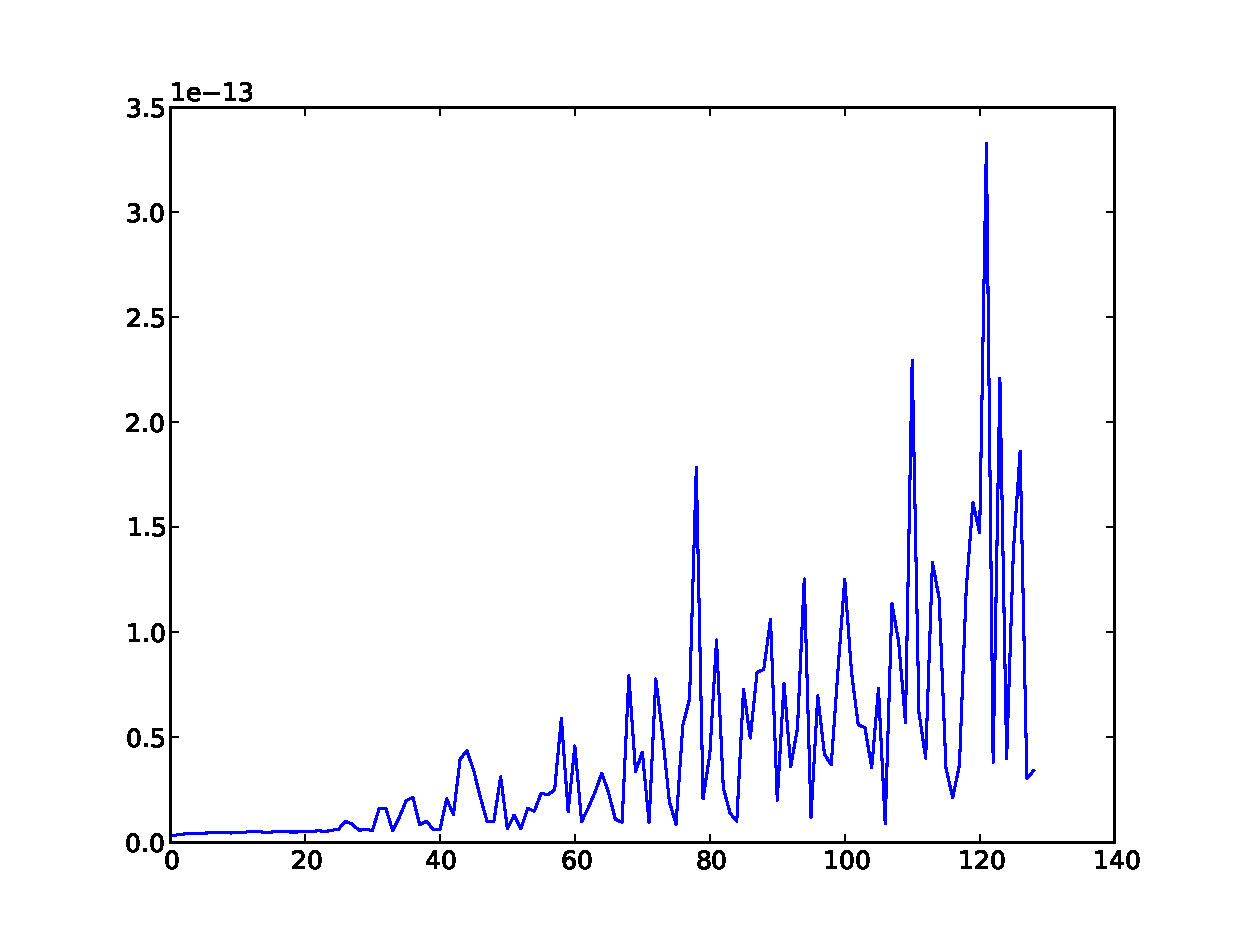
\includegraphics[scale=0.7]{Figures/exact_numerical_2d_n130.eps}
 \caption[Numerical exact error plot FE in 2D]{Numerical solution from the FE scheme versus the exact numerical solution of the FE scheme in 2D. 
 Parameters of importance are $\Delta t$ which is almost on the stability criterion, $\Delta t = \frac{\Delta x \Delta y}{5} = 8\cdot10^{-5}$ and the diffusion coefficient $D$ which must be $D = \frac{1}{2}$ in order to fulfill the diffusion equation.}
 \label{exact_numerical_2d_n130}
\end{figure}

\subsubsection{The BE scheme}
For the BE scheme the exact numerical solution is more implicit than for the FE scheme. 
As for the FE scheme, the numerical exact solution is simply the solution to the difference equation that the PDE is rewritten as. 
However, the BE scheme is implicit and results in a system of linear equations. 
This was derived in section \ref{discretizing} and the resulting linear system is

\begin{equation*}
 \mathbf M \vec u^{n+1} = \vec u^n
\end{equation*}

The solution to this linear system is trivial
\begin{equation*}
 \vec u^{n+1} = \mathbf M^{-1} \vec u^n
\end{equation*}

though it is an inefficient way of solving the system in this case. 
As indicated in section \ref{discretizing} all the information about the system lies in the mass matrix $\mathbf M$, and this matrix must be carefully assembled. 
It is then preconditioned and the system is solved by the ``tridiag'' solver mentioned earlier. 
In principle this is the same as doing and storing the inverse of $\mathbf M$ and then multiplying this inverse by the solution at the previous time-step. 
Another way of doing this is by raising $\mathbf M$ to the required power and then doing the multiplication with the initial condition as stated in equation \eqref{BE_numex}.

\begin{equation}\label{BE_numex}
 \vec u^{n+1} = \left(\mathbf M^{-1}\right)^{n+1} \vec u^0
\end{equation}

Equation \eqref{BE_numex} is the numerical exact solution to the BE scheme, but it has a few problems compared to the exact solution to the FE scheme. 
Testing is done by storing the inverse of the assembled matrix, solving eq. \eqref{BE_numex} for the desired number of steps and comparing the solution with the result of a simulation. 
The problem with this approach is that the inverse of $\mathbf M$ gives a lot of round off errors, especially with entries of $10^{-20}$ and smaller. 
These entries would be zero if the analytical inverse was taken, but are clearly not zero in the matrix. 
Terms of this magnitude give rise to a lot of potential uncertainty, and the result is that the desired accuracy must be reduced. 
Figure \ref{numex:BE1D} shows the accuracy of the simulation compared to the result of a simulation with the BE discretization. 
Although the accuracy is some $5$ orders of magnitude worse than the numerical exact for the FE scheme, it is still not too bad. 

\begin{figure}[H]
 \centering
 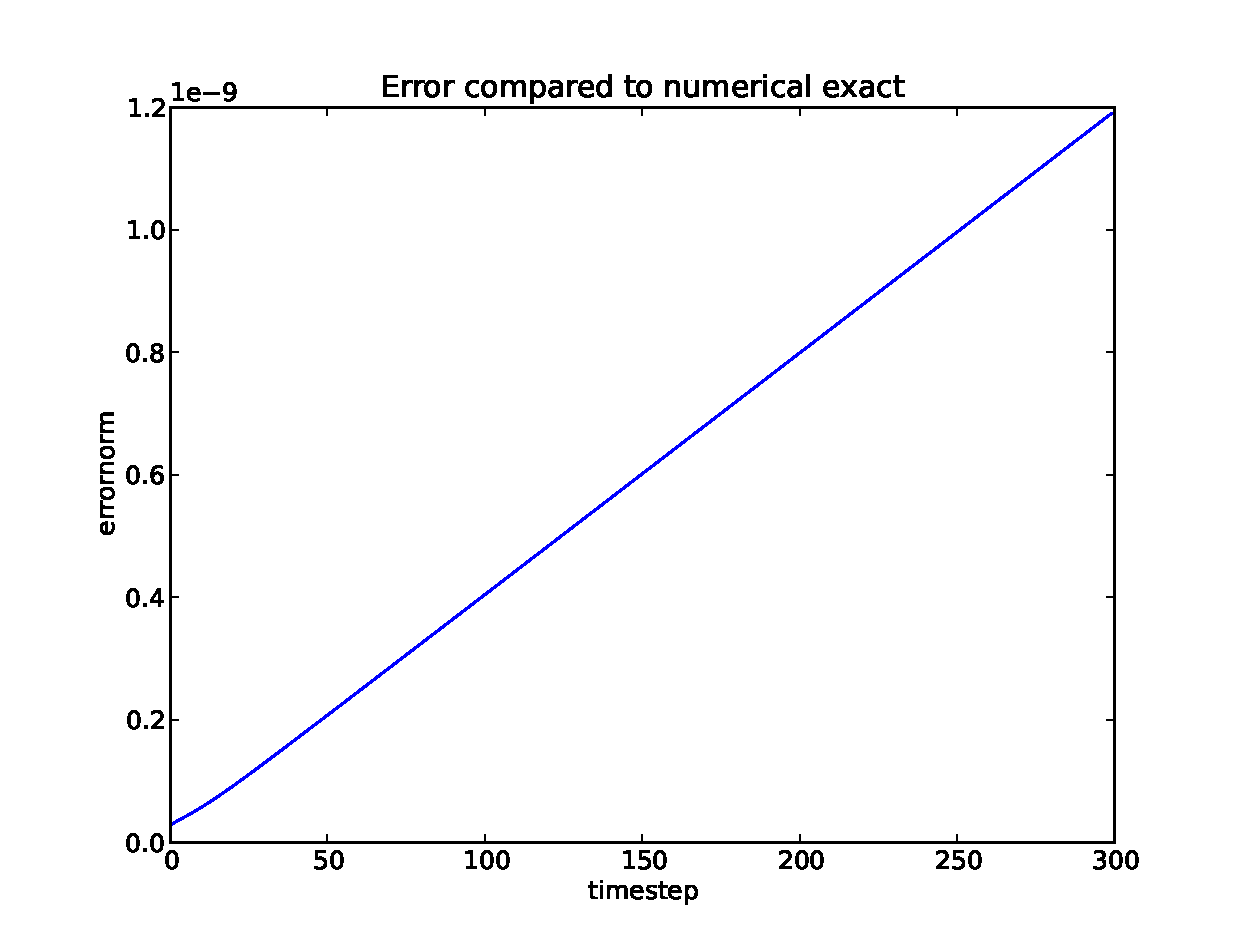
\includegraphics[scale=0.7]{../doc/results/experiment_14042014_0759_BE1D_numerical_exact/results/numerical_exact.eps}
 \caption[Numerical exact errorplot for BE scheme]{Error plot showing the norm of the difference between the numerical exact solution for the BE scheme in 1D (eq. \ref{BE_numex}) and a simulation. 
 The error is not machine precision, but significantly smaller than $\Delta t$ which for this simulation is $\Delta t=0.01$. 
 This increased error most likely originates in the many roundoff errors in the inverted matrix where a lot of terms which analytically would be zero are represented as $10^{-16}$ and smaller.}
 \label{numex:BE1D}
\end{figure}

A nice property of the numerical exact solution to the BE scheme is that it generalizes to the 2D scheme. 
Figure \ref{numex:BE2D} shows the accuracy of the BE scheme when compared to its numerical exact solution. 
As for the 1D case, there will be some round-off errors which will have an effect on the accuracy. 

\begin{figure}[H]
 \centering
 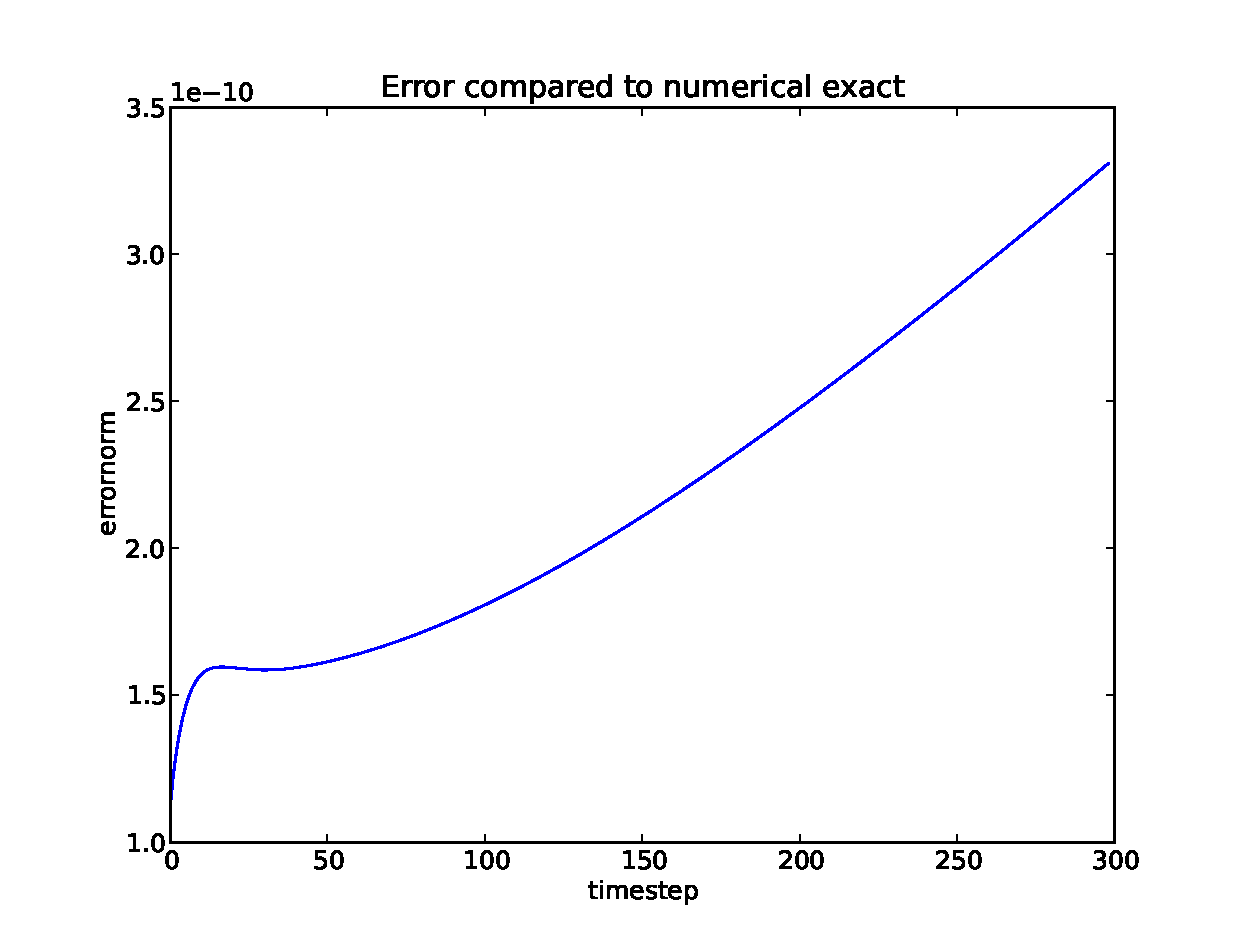
\includegraphics[scale=0.5]{../doc/results/experiment_30042014_0914_BE2D_numex/results/numerical_exact.eps}
 \caption[Numerical exact errorplot for BE scheme in 2D]{Error plot showing the norm of the difference between the numerical exact solution for the BE scheme in 2D (eq. \ref{BE_numex}) and a simulation. 
 The error is not machine precision, but significantly smaller than $\Delta t$ which for this simulation is $\Delta t=0.01$. 
 This increased error most likely originates in the many roundoff errors in the inverted matrix where a lot of terms which analytically would be zero are represented as $10^{-16}$ and smaller.}
 \label{numex:BE2D}
\end{figure}

% \clearpage

\section{Testing the Random walk implementation}\label{testing_random_walks}


The RW implementation will be verified using the same techniques that were used to verify the PDE solvers with the exception of a numerical exact solution since there is none. 
However, the initial condition used for the PDE solvers cannot be represented to a satisfying accuracy by a distribution of walkers. 
A Heaviside step function on the other hand can be perfectly represented by said distribution and is defined in equation \eqref{Heaviside_def}. 


\begin{equation}\label{Heaviside_def}
 H(x-a) = \begin{cases}
           1\;\;x\geq a\\
           0\;\;x<a
          \end{cases}
\end{equation}
In order to verify the RW implementation an initial distribution of walkers which follows the Heaviside step function is given to the program, and a simulation is run for some number of time steps. 
An exact solution must also be found to the diffusion equation (eq. \ref{simple_diffusion_equation}) for error calculations and this is done by separation of variables. We have

\begin{align}
 \frac{\d u}{\d t} &= D\frac{\d^2 u}{\d x^2}\\
 \frac{\d u(0,t)}{\d x} &= \frac{\d u(1,t)}{\d x} = 0 \\
 u(x,0) &= H\left(x-\frac{1}{2}\right)\\
 D &= 1
\end{align}
and
\begin{align*}
 u(x,t) = F(x)T(t) \implies \frac{T'(t)}{T(t)} = \frac{F''(x)}{F(x)}
\end{align*}
where the primes denotes the respective derivatives. We separate the equation using a separation constant $\lambda$
\begin{align*}
 T'(t)-\lambda T(t) &= 0 \\
 \implies T(t) &= C\exp(\lambda t)\\
 F''(x) -\lambda F(x) &= 0 \\
 \implies F(x) &= C_1\exp(\sqrt{\lambda}x) + C_2\exp(-\sqrt{\lambda}x)
\end{align*}
where $C$, $C_1$ and $C_2$ are arbitrary constants. 
Choosing $\lambda = -\mu^2$ lets us rewrite the spatial solution in terms of sines and cosines. 
There are really three choices here; $\lambda = -\mu^2$, $\lambda = \mu^2$ and $\lambda = 0$, but the first is chosen because the results of the other choices are unphysical or uninteresting. 
Inserting $\lambda = -\mu^2$ into the expression found for $F(x)$ gives

\begin{equation*}
 F(x) = a\cos(\mu x) + b\sin(\mu x)
\end{equation*}

The boundary conditions result in
\begin{align*}
 F'(0)T(t) = F'(1)T(t) = 0
\end{align*}

Since the time dependent solution cannot be exactly zero and is independent of position by construction ($C\exp(\lambda t)|_{x=0} = C\exp(\lambda t) \neq 0$), the first derivative of the spatial solution must be zero at the boundaries
\begin{align*}
 F'(x) &= -a\mu\sin(\mu x) + b\mu\cos(\mu x) \\
 F'(0) &= -a \mu\sin(0) + b\mu\cos(\mu x) \\
 &= b\mu\cos(\mu x) \implies b=0 \\
 F(1) &= a\cos(\mu) \implies \mu = n\pi
\end{align*}
Which suggests that a Fourier series in cosines is the solution to the equation, and it will look like this.
\begin{equation}
 u(x,t) = a_0 + \sum\limits_{n=1}^\infty a_n\exp\left(-(n\pi)^2t\right)\cos(n\pi x)
\end{equation}

The coefficients are found by approximating the initial condition
\begin{align*}
 a_0 &= \int\limits_0^1H(x-0.5)dx = \frac{1}{2} \\
 a_n &= 2\int\limits_0^1H(x-0.5)\cos(n\pi x)dx \\
 &= 2\int\limits_{0.5}^1\cos(n\pi x)dx \\
 &= \frac{2}{n\pi}\left[sin(n\pi x)\right]_{0.5}^1 \\
 &= \frac{2}{n\pi}\sin(n\pi) - \sin(\frac{n\pi}{2}) \\
 &= \frac{2\sin(\frac{n\pi}{2})}{n\pi}\\
 a_n &= \frac{2}{\pi m} (-1)^m\;\;;\;\; m=2n+1
\end{align*}
which gives us the final solution
% \begin{equation}
%  u(x,t) = \frac{1}{2} + \sum\limits_{n=1}^\infty \frac{2\sin(\frac{n\pi}{2})}{n\pi}e^{-(n\pi)^2t}\cos(n\pi x)
% \end{equation}
\begin{equation}
 u(x,t) = \frac{1}{2} + \sum\limits_{m=0}^\infty \frac{2(-1)^m}{m\pi}e^{-(m\pi)^2t}\cos(m\pi x)
\end{equation}
This is the manufactured solution the simulations will be tested against for the verification of the RW implementation.

%%%%%%%%%%%%%%%%%%%%%%%%%%%%%%%%%%%%%%%%%%%%%%%%%%%%%%%%%

A convergence test can now be performed to find the convergence rate for the random walkers.
It will be slightly modified by testing for the number of walkers rather than the time step. 


Using the maximum of the error measure already in use, the convergence rate has been tested for the following measures of Hc:
\begin{lstlisting}
 Hc = [200,1400,5600,10400,32000]
\end{lstlisting}

The convergence test suggests that the convergence rate for random walks follows the proportionality in equation \eqref{convergence_rate_RW}. 
\begin{equation}\label{convergence_rate_RW}
err \propto Hc^{\frac{-1}{2}}
\end{equation}
This relation says that while increasing the number of walkers will in fact reduce the error, the convergence is very slow. 
Should we wish to do so, we can force the error to $\mathcal{O}(\Delta t^2)$, but this will be extremely inefficient. In fact we can find the relation as $Hc\sim\Delta t^{-2}$ for $\epsilon\sim\mathcal{O}(\Delta t)$, and $Hc\sim\Delta t^{-4}$ for $\epsilon\sim\mathcal{O}(\Delta t^2)$. 
Clearly there will be enough trouble for the simpler cases...



\begin{figure}[H]
 \centering
 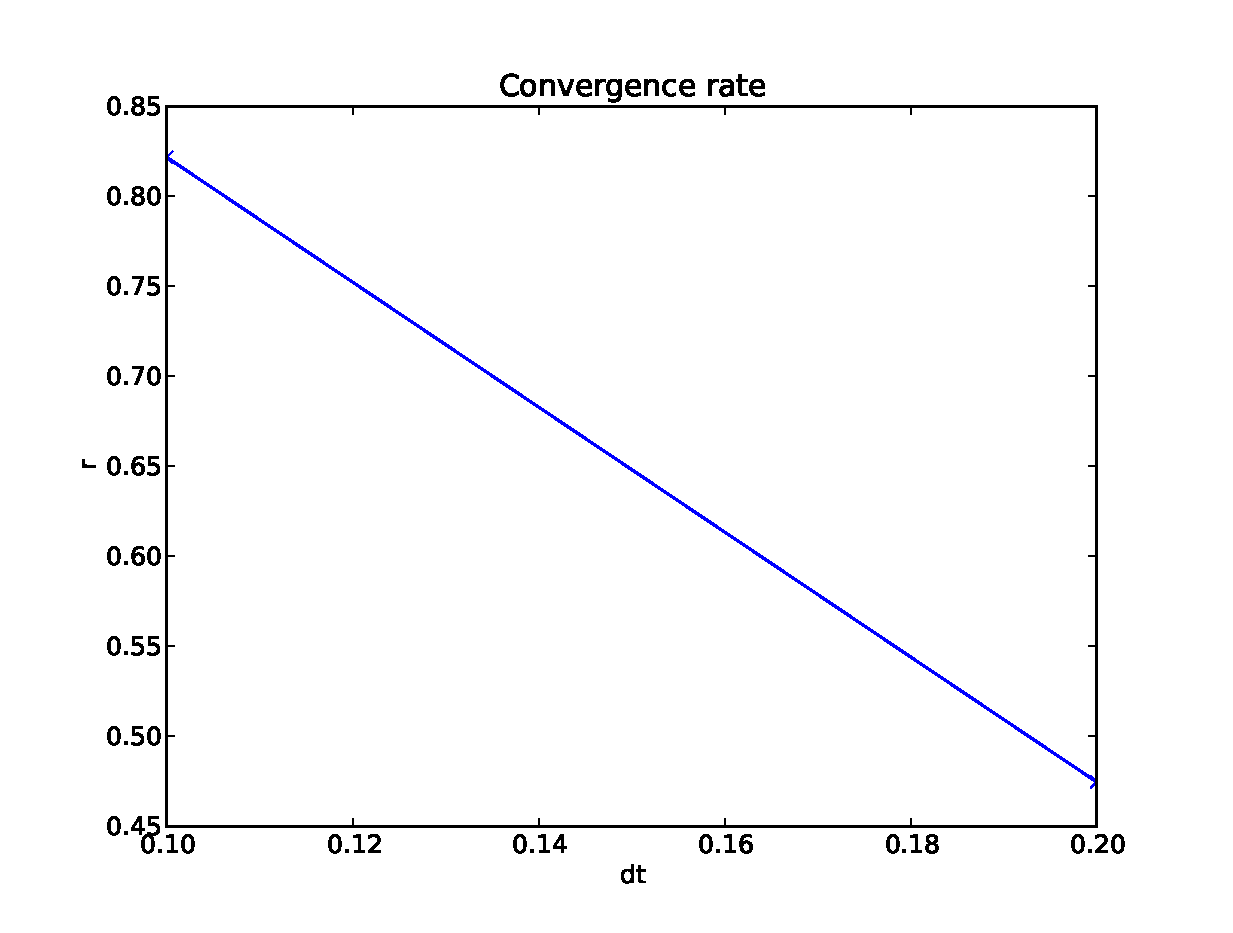
\includegraphics[scale=0.7]{../doc/results/experiment_18022014_1413_RW_convergencetest_1d/ConvergenceTest.eps}
 \caption[Convergence test RW]{A convergence test for the isotropic random walk implementation using different conversion factors, Hc. The x axis (conversion rate) is log transformed and ranges from 100 to 50000 in real numbers.}
 \label{ConvergenceTestRW}
\end{figure}
\begin{figure}[H]
 \centering
 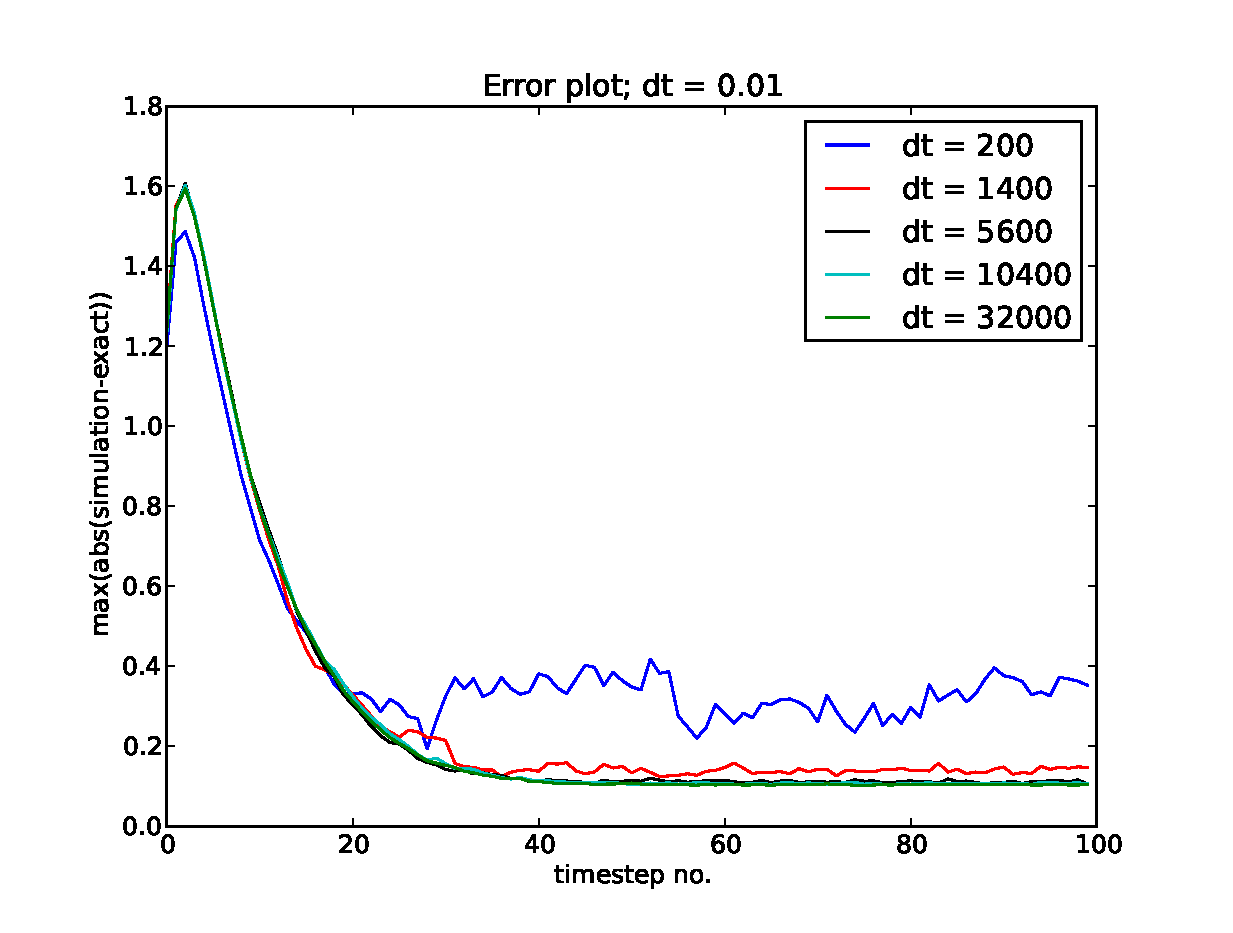
\includegraphics[scale=0.7]{../doc/results/experiment_18022014_1413_RW_convergencetest_1d/results/errorplot.eps}
 \caption[Error plot RW]{An error plot for the same simulation as in figure \ref{ConvergenceTestRW}. The $\Delta t$ in question is used to couple the RW simulation and the exact solution. For each $\Delta t$ the RW simulation does 100 steps with a step length calculated from equation \eqref{steplength}}
\end{figure}




\section{Testing the combined solution}

This section will test how combining the RW model with the PDE model affects the error, and whether it is possible to make the error term have first order convergence.
As will be discussed in chapter \ref{Software:About} there are many candidates as to the combination of the solutions, but it turns out that simply replacing the solution in the relevant area with the solution from a RW simulation before the PDE integration is done is sufficient. 
\begin{quotation}
 A scientific theory should be as simple as possible, but no simpler
\end{quotation}
It will therefore be unnecessary to add any fancy curve fitting when it is not needed. 

Before we start with the verification, however, a simplified problem which in principle is the same as the diffusion - RW problem, will be presented.

\subsection{A simplified version of the algorithm}\label{simplified_test}

Monte Carlo (MC\nomenclature{MC}{Monte Carlo}) methods are immensely important in modern computational science (\emph{reference}), and can be used to solve integrals as well as random walks. 
As a simplified analogy to our method for solving the diffusion equation we ca look to the Ordinary Differential Equation (ODE) in equation \eqref{ODE}. 
\begin{equation}\label{ODE}
 \frac{\d f}{\d x} = g(x)\;\text{,}\; x\in [a,c]
\end{equation}
Equation \eqref{ODE} is easily solvable (see eq. \eqref{ODE_solution}). For the sake of illustration we also specify that $g(x) = \frac{1}{x}$ and divide the integral in two parts, introducing $b\in (a,c)$.
\begin{equation}\label{ODE_solution}
 f(x) = \int\limits_a^b g(x)\,dx + \int\limits_b^c g(x)\,dx
\end{equation}
This is a case where we have complete control over all parts of the solution which is $f(x) = f(b)-f(a) + f(c)-f(b)$, and we can solve the two parts of the integral in two different ways; by the midpoint method and by MC integration, respectively. The convergence rates of these methods are $2$ and $0.5$ respectively. 
By the relation found in chapter \ref{theory:changing_between_lenghtscales} (eq. \eqref{definition_Hc_first}) the number of MC samples should be proportionate to the resolution used by the midpoint-rule to the power of four. 
\begin{align*}
 \frac{1}{\sqrt{N}} \simeq \Delta x^2 \\
 N \simeq \frac{1}{\Delta x^4} = N_x^4
\end{align*}
The following output is from a program (donated) by Hans Petter Langtangen which does the required integration and calculates the convergence rates. 
It uses the relation described, but multiplies with a constant, giving us 
\begin{equation}\label{num_walkers_MC_integration}
 N = 2000\times N_x^4
\end{equation}
\clearpage
\begin{lstlisting}
  N_x	      N_MC	        error       MC_error   MP_error
   1        2000 (   1)  2.650E-02   2.648E-02   2.391E-05
   2       32000 (   1)  7.392E-03   7.433E-03  -4.136E-05
   4      512000 (   1)  1.918E-03   1.927E-03  -8.954E-06
   8     8192000 (   8)  4.683E-04   4.866E-04  -1.832E-05
  16   131072000 ( 131)  1.176E-04   1.220E-04  -4.320E-06
  
  Convergence rates
total    MP    MC
-1.84 -1.83  0.20
-1.95 -1.95 -0.55
-2.03 -1.99  0.26
-1.99 -2.00 -0.52
\end{lstlisting}
The convergence rate for the whole integral is roughly $2$ which is what we expect. This suggests that the idea behind the algorithm is sound. \\
Another thing to notice is the convergence rate of the MC method which is sort off all over the place, this illustrates how difficult it is to verify the simulations. 
As the listed output and equation \eqref{num_walkers_MC_integration} shows, the number of walkers or MC samples grows very fast making it computationally very demanding to do the calculations.

\subsection{Introducing walkers}


First of all, using random walkers on parts of the mesh will have a considerable, negative impact on the error estimate. 
As we have discussed before, the solution from the random walkers will fluctuate around the ``correct'' (it is in fact correct while verifying) solution with amplitude proportional to $\frac{1}{\sqrt{N_{ij}}}$ which will depend on the PDE-solution in the mesh-point. 
It will also, as demonstrated in chapter \ref{simplified_test}, be possible to force the combined solution to have the desired properties in terms of error-estimates but at considerable computational cost. 
The various error tests will therefore be carried out using only the implicit scheme since the time-step can be chosen more freely, thus reducing the required number of walkers.\\
Keeping in mind that the spatial error goes like $\Delta x^2$ the time-step should be chosen so that $\Delta t> \Delta x^2$ to make sure the error from the time derivative is dominant. 
Figure \ref{combined_BE1d} shows the results of a test where $\Delta x$ was fixed at $\frac{1}{100}$ and both the time step and the conversion rate for walkers were improved over three simulations. 
The figure shows that most of the fluctuations are irrelevant in the beginning of the simulation, but the become increasingly more important as steady state is reached. 
A convergence rate of 1 is also reached, suggesting that the walkers are converging to the PDE solution. 

% \begin{figure}[H]
% %  This figure shows how the simulations behaved before the order of integration was changed (in 2d)
%  \centering
%  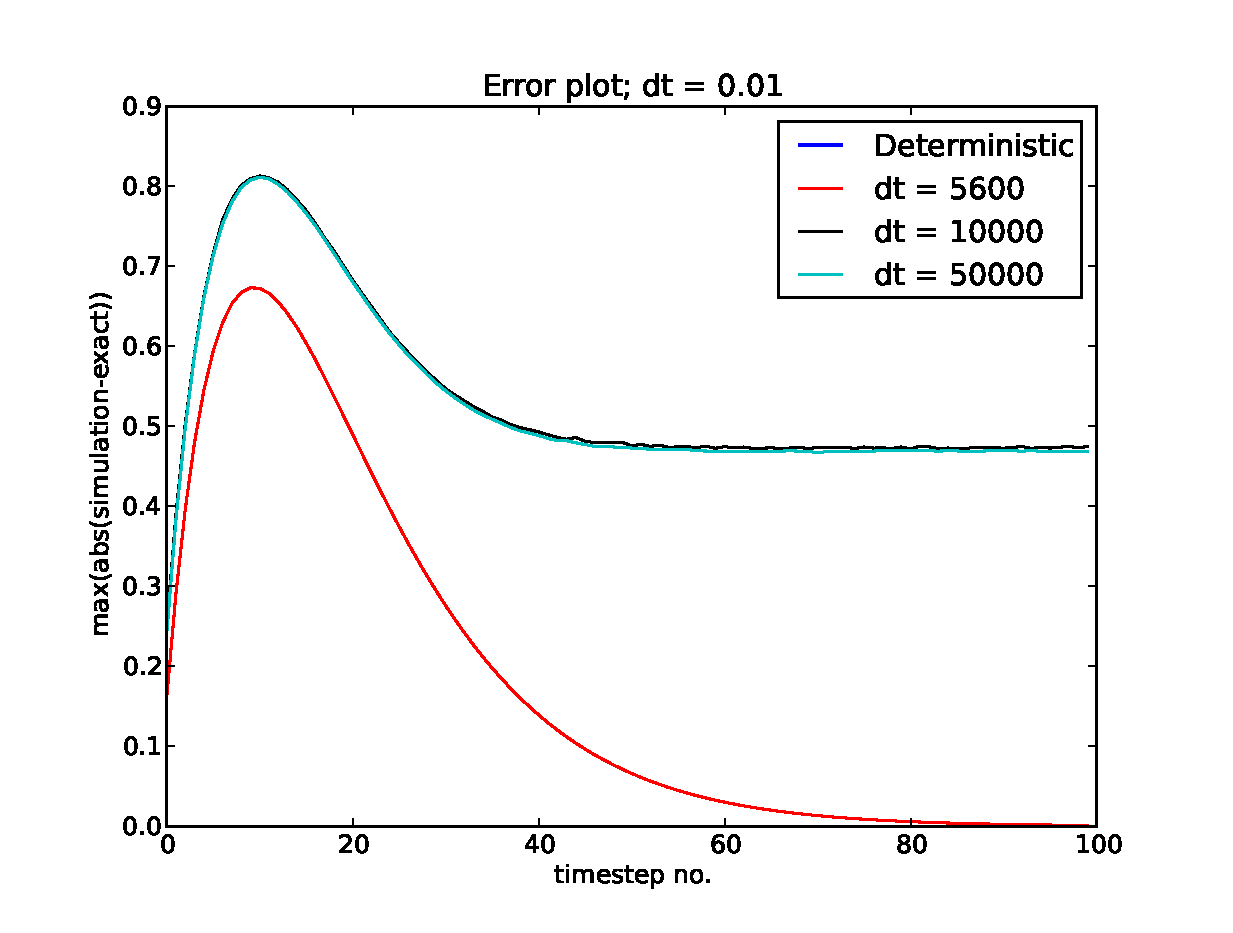
\includegraphics[scale=0.7]{../doc/results/experiment_17022014_1541/results/errorplot.eps}
%  \caption{Error-plot of the combined solution using an increasing number of walkers. Parameters of importance are $\Delta t = 0.01$, $\Delta x = \frac{1}{75}$. Simulations done with the BE scheme for 100 steps.}
%  \label{errorplot_combined_BE2d}
% \end{figure}

\begin{figure}[H]
 \centering
 \begin{subfigure}[b]{0.48\textwidth}
 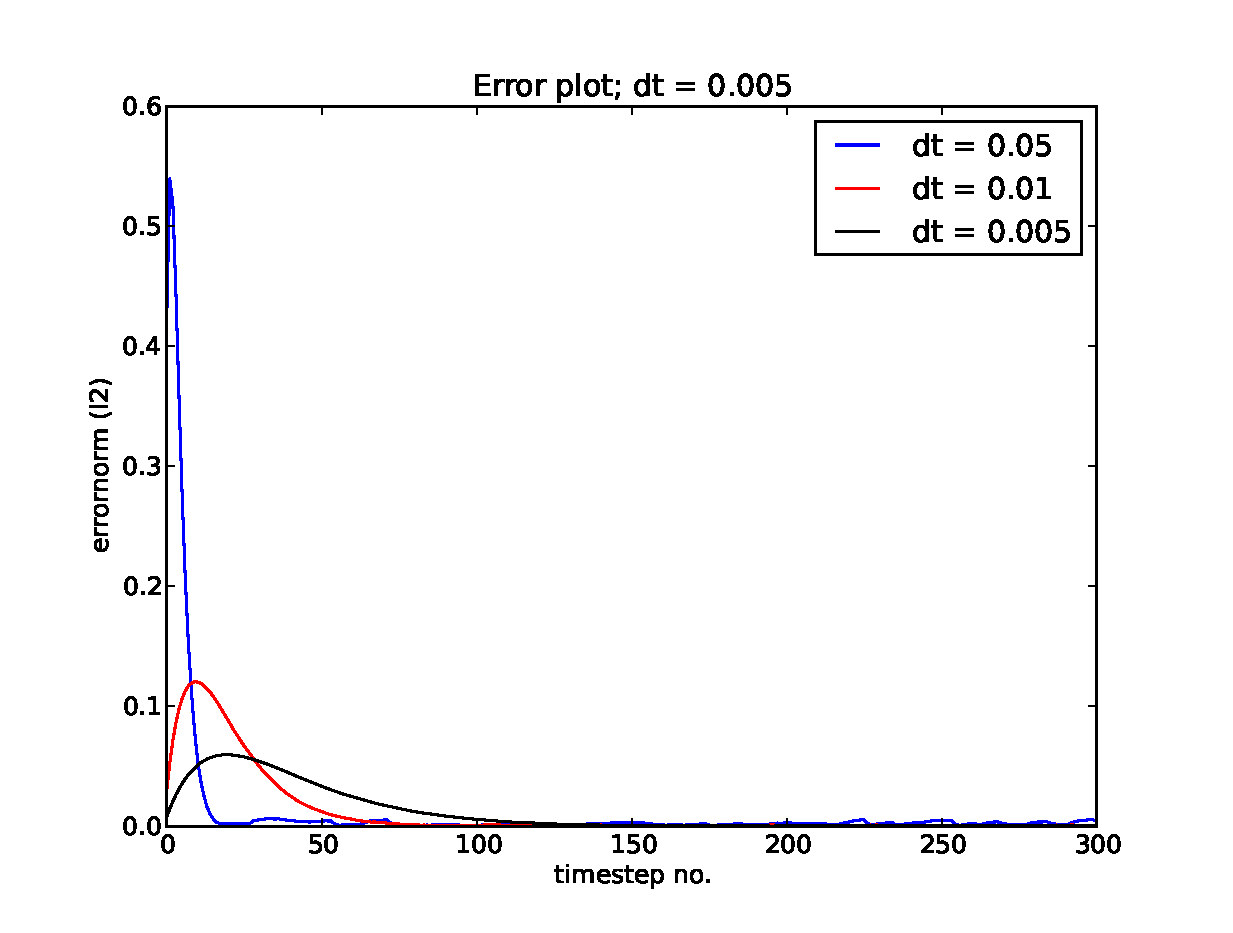
\includegraphics[width=\textwidth]{../doc/results/experiment_15042014_0608_convergence_tests_etc/results/errorplot.eps}
\caption{}  
 \label{combined_BE1d:errorplot}
 \end{subfigure}
 \begin{subfigure}[b]{0.48\textwidth}
  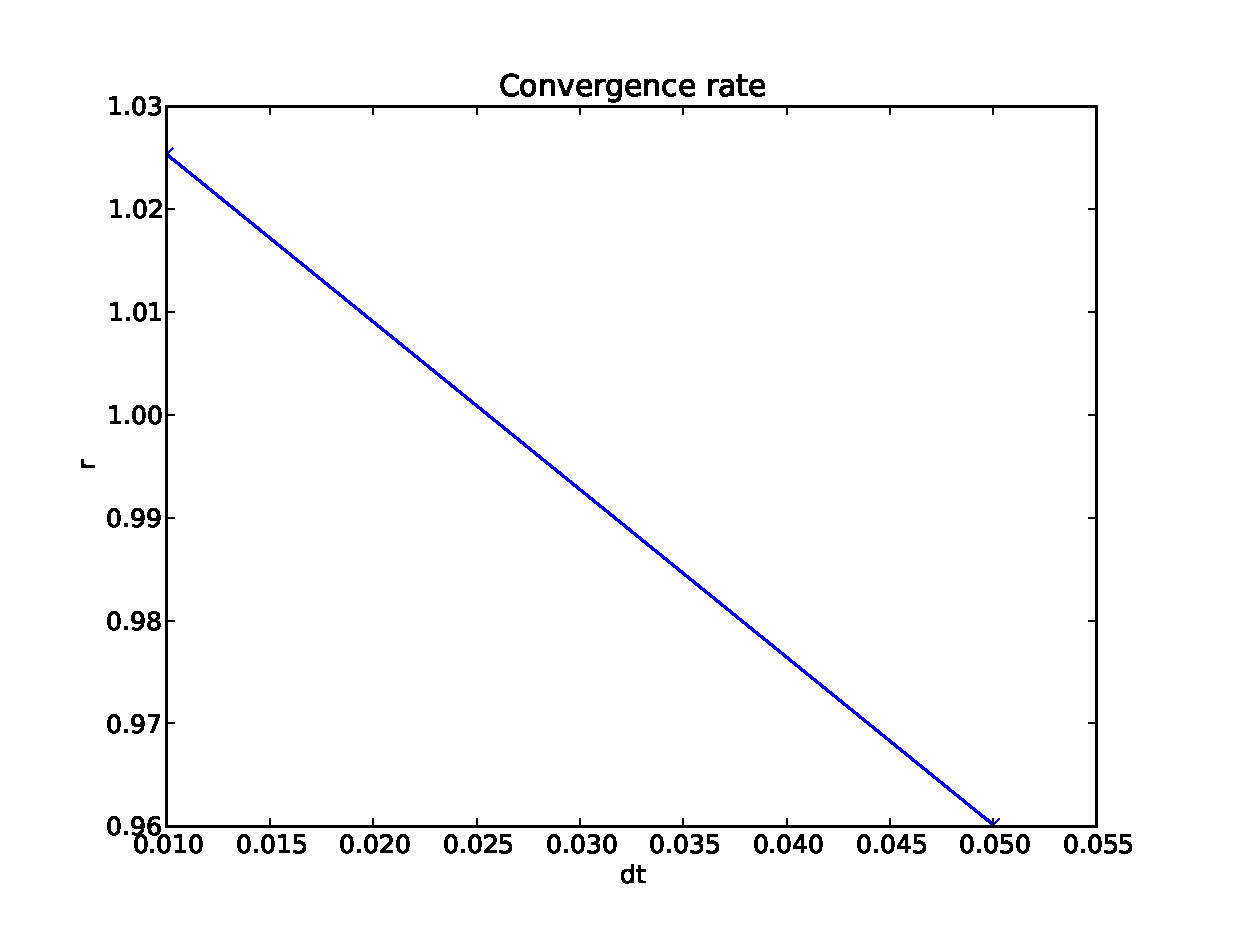
\includegraphics[width=\textwidth]{../doc/results/experiment_15042014_0608_convergence_tests_etc/results/ConvergenceTest.eps}
  \caption{}
   \label{combined_BE1d:convergence}
 \end{subfigure}
 \caption[Error test for BE combined with RW in 1D]{\ref{combined_BE1d:errorplot} shows the error plot for a test where $\Delta x$ was fixed at $\Delta x = \frac{1}{100}$ and $\Delta t$ was reduced from $0.05$ to $0.01$ and finally to $0.005$. 
 The conversion rate, $Hc$ was updated for each simulation to have the value $Hc = \frac{1}{\Delta t^2}$, meaning the error from the walkers should be smaller than the error from the time derivative. 
 Walkers are placed on 10\% of the mesh from $x=0.4$ to $x=0.5$. 
 \ref{combined_BE1d:convergence} shows the convergence rate in time for the same test.}
 \label{combined_BE1d}
\end{figure}

%%%%%%%%%%%%%%%%%%%%%%%%%%%%%%%%%%%%%%%%%%%%%%%%%%%%%%
%% Rewrite from here down, and redo the experiments %%
%%%%%%%%%%%%%%%%%%%%%%%%%%%%%%%%%%%%%%%%%%%%%%%%%%%%%%


\subsection{Increasing the time step and the relative size of walk-area}\label{increasing_dt}

Now that we have an estimate of how to adjust the step length of the walkers in order to adjust for the time step, $\Delta t$, on the PDE level we would like to investigate the actual effects of running the simulation with a larger time step to verify our calculations. 
First off all, Figure \ref{errorplot_BE1D_noWalk} shows the error norm of a simulation of the simplest diffusion equation \eqref{simple_diffusion_equation} discretized by the BE scheme using a time step which would make the FE discretization unstable (There is something strange about its convergence). 
Figure \ref{errorplot_BE1D_Walk} shows the same simulation for various conversion parameters for the random walk. 
These simulations have input from the random walk model on some 20\% of the mesh points. 
As a comparison Figures \ref{errorplot_BE1D_walk_5_percent} and \ref{errorplot_BE1D_walk_35_percent} have 5\% and 35\% of the mesh points affected by walkers. 
An interesting property of both these figures is the instability in the error for very low conversion factors. 
\emph {There seems to be a limit as to how large of an inaccuracy the scheme can handle and still produce meaningful results. }
Another thing to notice from these figures is that a larger relative area of walkers implies more walkers are required in order to make the scheme as exact as it will get. 
Apparently, the introduction of walkers will give an increased error no matter how many are used.

\begin{figure}[H]
\centering
\begin{subfigure}[b]{0.48\textwidth}
% 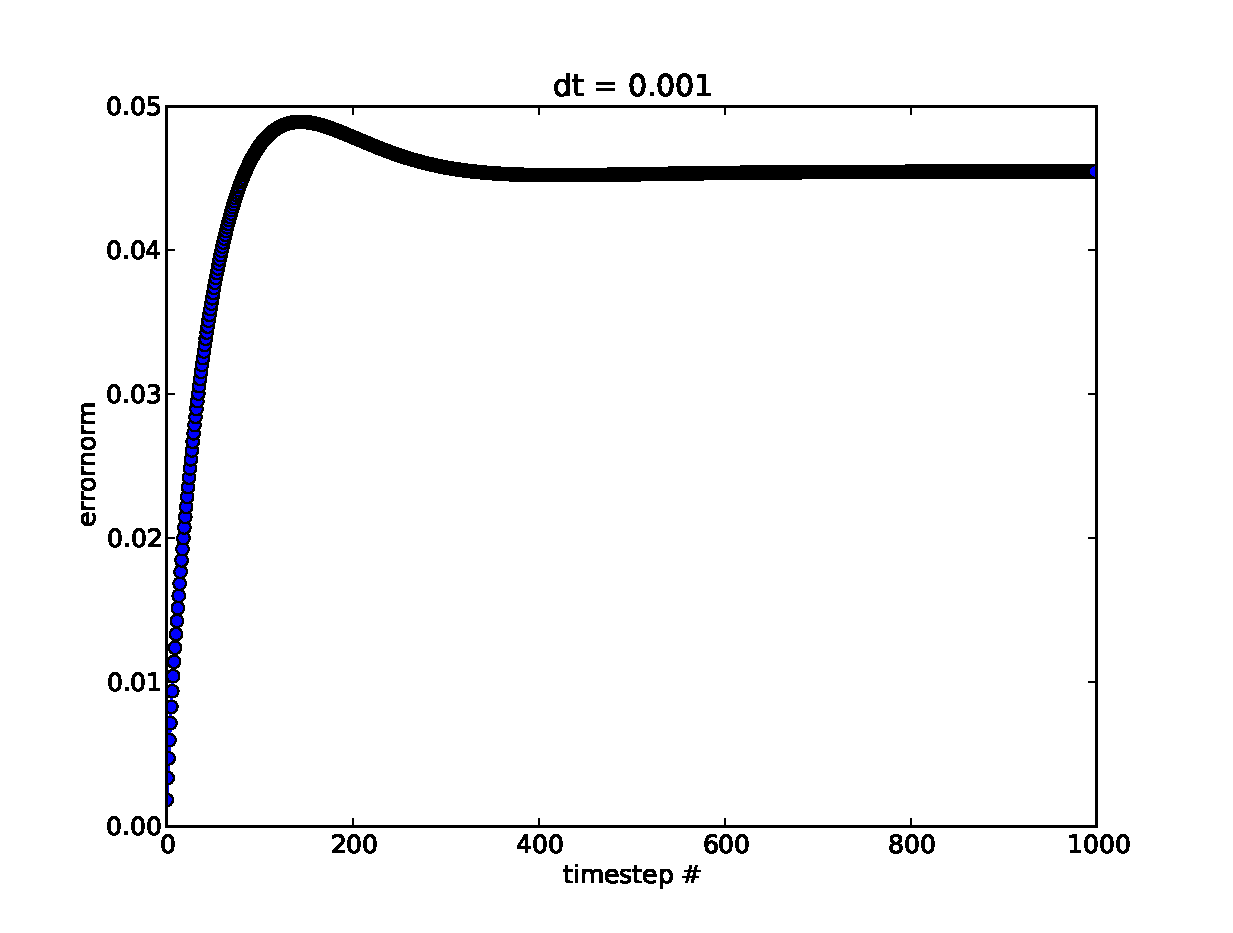
\includegraphics[width=\textwidth]{../doc/results/experiment_19112013_1514/results/deterministic_errorplot.eps}
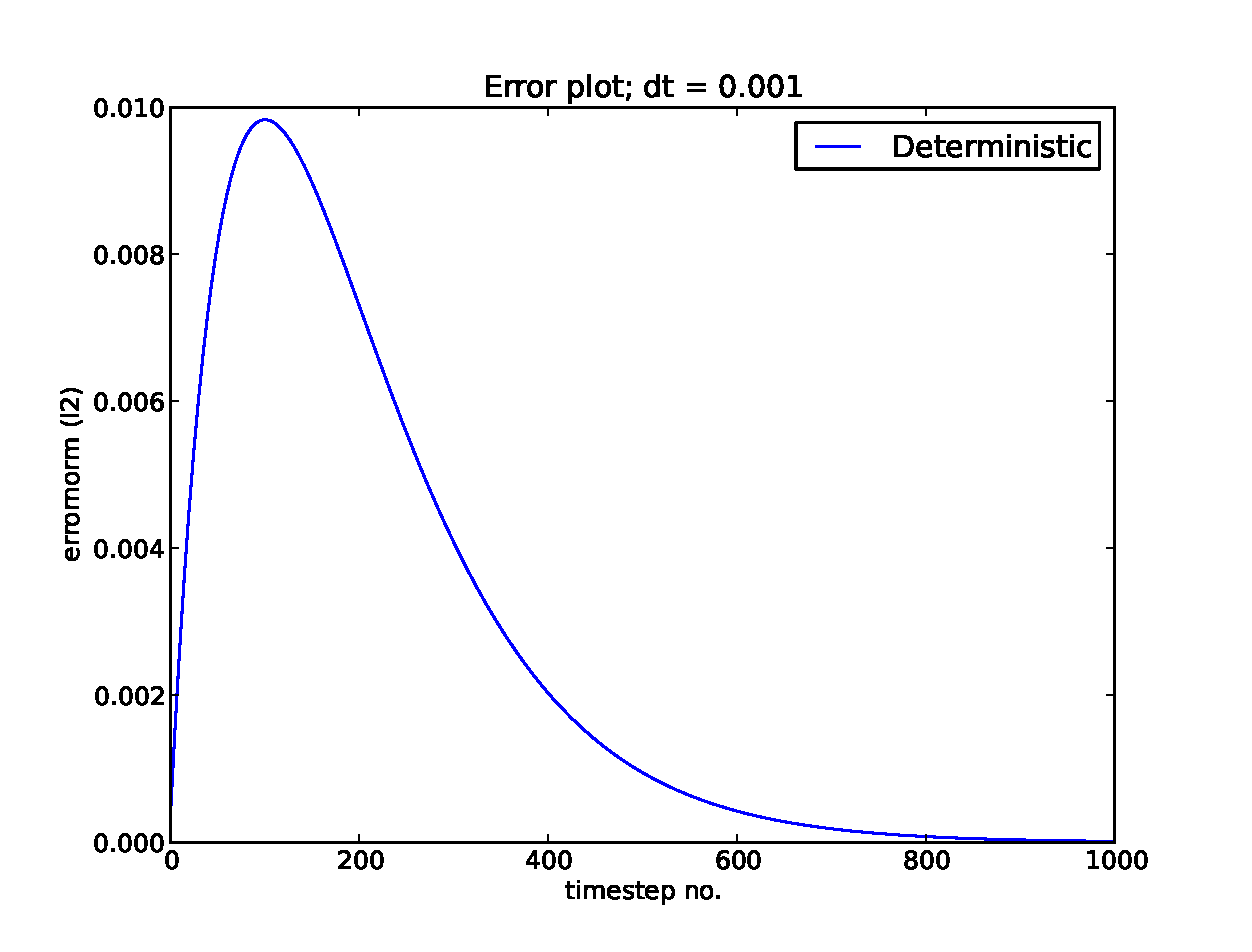
\includegraphics[width=\textwidth]{Figures/errorplot_BE1D_deterministic.eps}
\caption{}
\label{errorplot_BE1D_noWalk}
\end{subfigure}
\begin{subfigure}[b]{0.48\textwidth}
%  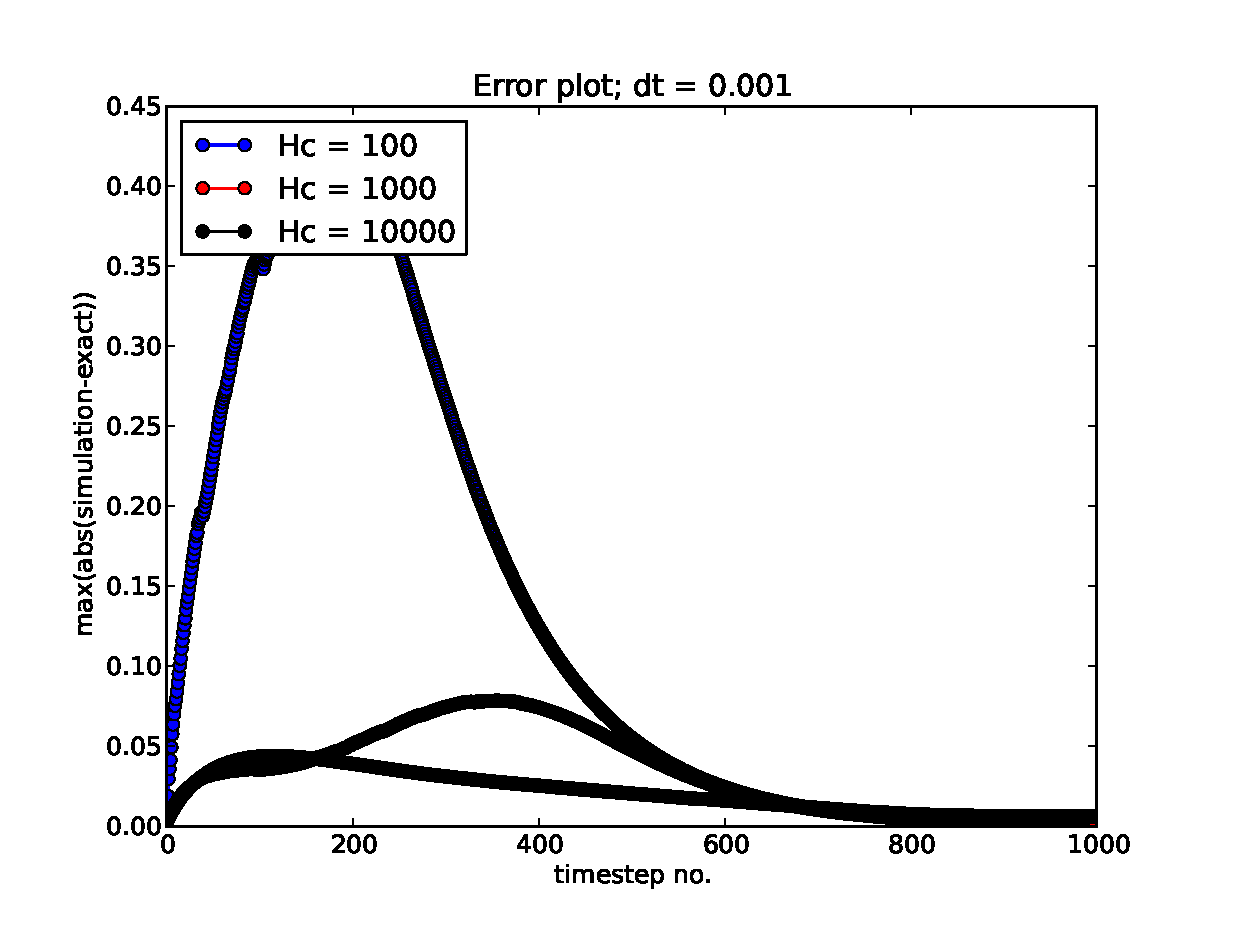
\includegraphics[width=\textwidth]{../doc/results/experiment_19112013_1514/results/errorplot.eps}
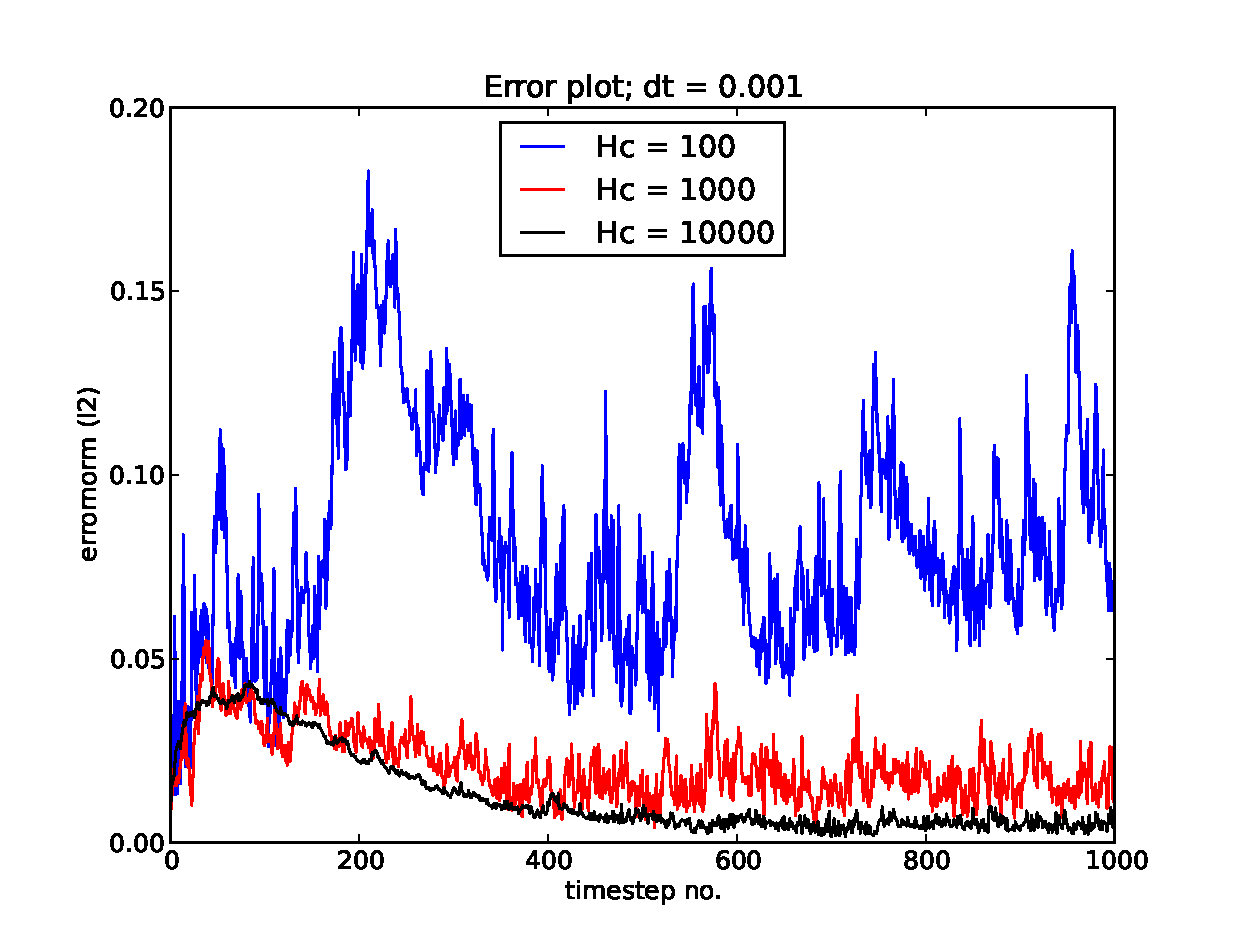
\includegraphics[width=\textwidth]{Figures/errorplot_BE1D_few_walkes.eps}
\caption{}
 \label{errorplot_BE1D_Walk}
\end{subfigure}
\caption[Error for 1D BE scheme with to few walkers]{Error for 1D BE scheme combined with RW solver using increasing number of walkers, but at most 1\% of the required number. In figure b there has been added walkers to the solution in the area $x\in[0.5,0.7]$ with $\Delta x = \frac{1}{50}$, which adds up to 20\% of the mesh. Compared to only the deterministic error in a, the 1\% simulation is not that bad.}
\label{errorplot_BE1D_first}
\end{figure}

\begin{figure}[H]
\centering
\begin{subfigure}[b]{0.48\textwidth}
 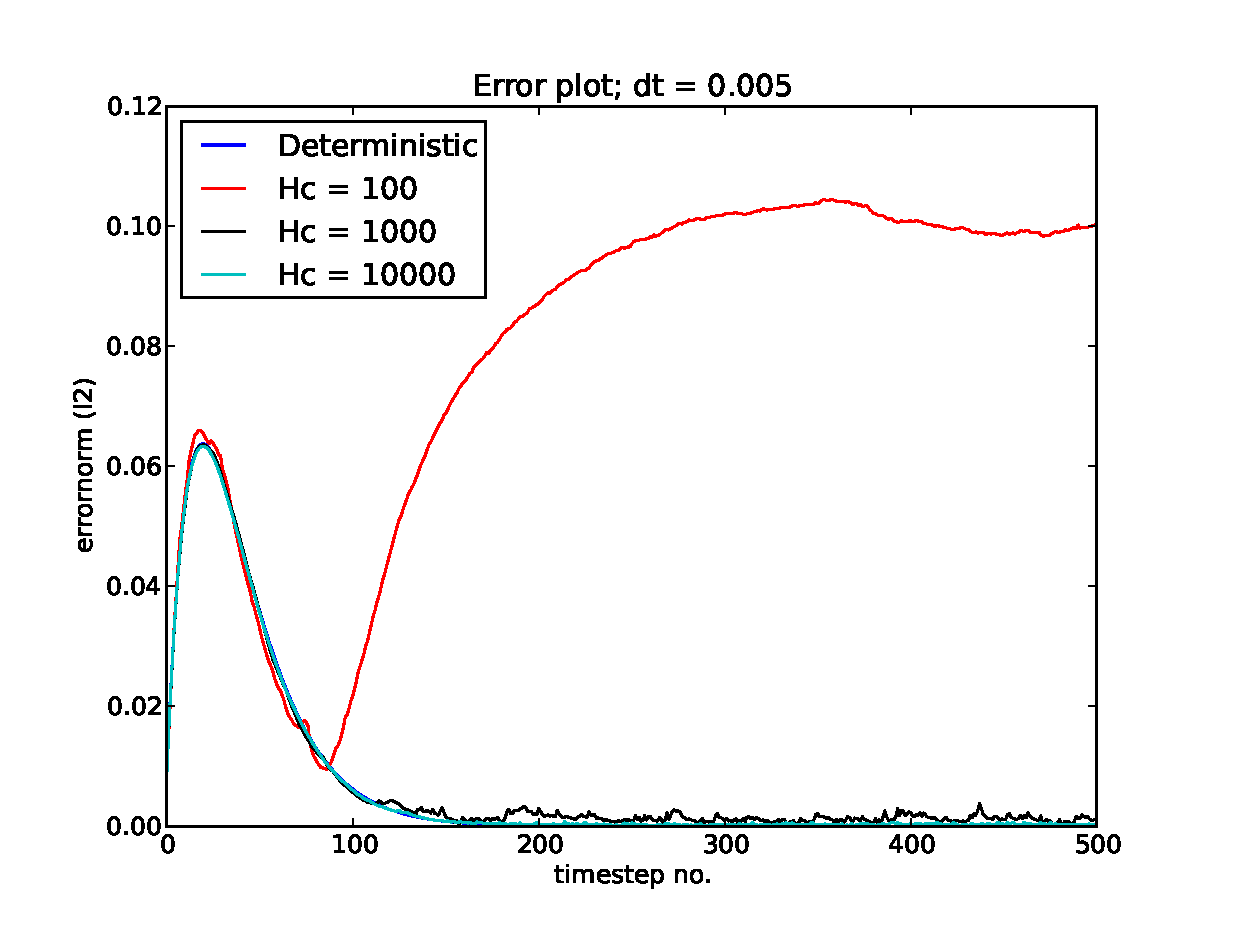
\includegraphics[width=\textwidth]{../doc/results/experiment_16042014_1139_convergence_tests_etc/results/errorplot.eps}
 \caption{Having walkers on 5\% of the mesh points.}
 \label{errorplot_BE1D_walk_5_percent}
\end{subfigure}
\begin{subfigure}[b]{0.48\textwidth}
 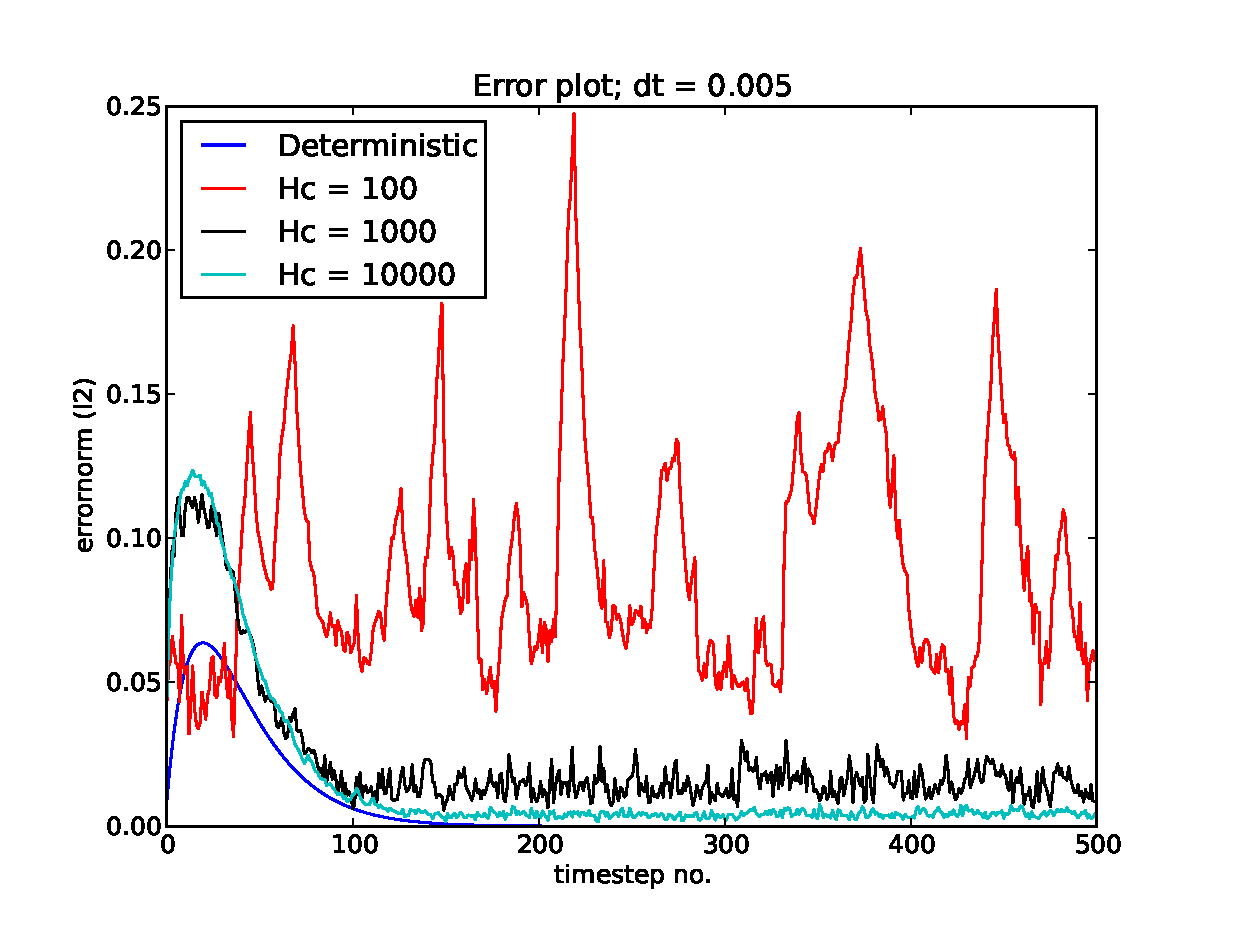
\includegraphics[width=\textwidth]{../doc/results/experiment_16042014_1202_tests_35percent_walkers/results/errorplot.eps}
 \caption{Having walkers on 35\% of the mesh points.}
 \label{errorplot_BE1D_walk_35_percent}
\end{subfigure}
\caption[Effects of increasing relative size of walk area]{The effect of increasing the size of the walk area for a fixed $\Delta t = 0.05$ and $\Delta x = 0.01$ using the BE discretization.}
\label{testing_walk_area_size_BE}
\end{figure}

The effects of changing the time step have also been investigated, and the results are shown in Figure \ref{testing_dt_size}. 
This test illustrates that the step length tweaking derived in section \ref{probability_distribution_and_timesteps} works since the error stabilizes around the size of $\Delta t$ and the fluctuations seem to be around $\sqrt{\frac{1}{N}}$ as predicted.\\

% Figure \ref{errorplot_BE1D_walk_large_dt} shows something a little bit unexpected. 
% Unlike almost all the other comparable plots, it seems that using the least amount of walkers gives the best result here. 
% This might be because the system quickly reaches its steady state, and will then be very well described by the continuum model. 
% Having a small conversion factor, Hc, will mean that very quickly there will be no walkers which sort of ruins the point. 
% This particular equation has steady state $u(t\to\infty,x) = 0$, and so not having any walkers will be perfect. 
% What we should read from this figure is rather that the simulation with the most walkers converges to an acceptable error, and that this is achieved just as fast as for the other two simulations.


\begin{figure}[H]
\centering
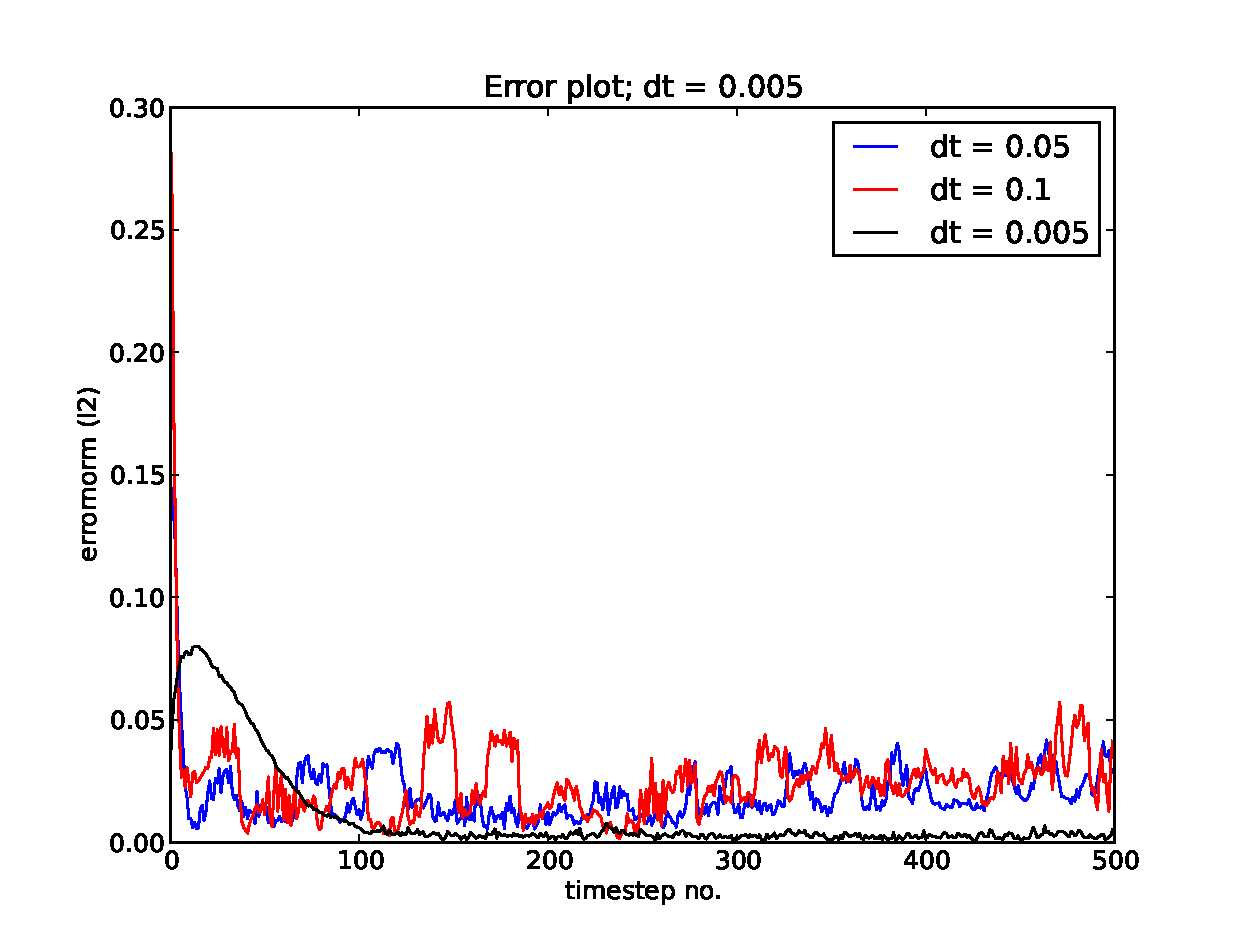
\includegraphics[scale=0.7]{Figures/errorplot_timestep_test.eps}
\caption[Effect of increasing time step]{Error norm of three tests where the spatial resolution was fixed at $\Delta x = \frac{1}{10}$ and the time step and conversion factor were changed. $\Delta t$ started at the stability criterion for the FE scheme $\Delta t = 0.5\cdot\Delta x^2$ and was increased up to $\Delta t = \Delta x$, maintaining the demand of $Hc = \frac{1}{\Delta t^2}$ for all the tests. }
\label{testing_dt_size}
\end{figure}
% \begin{figure}[H]
% \centering
% \begin{subfigure}[b]{0.48\textwidth}
%  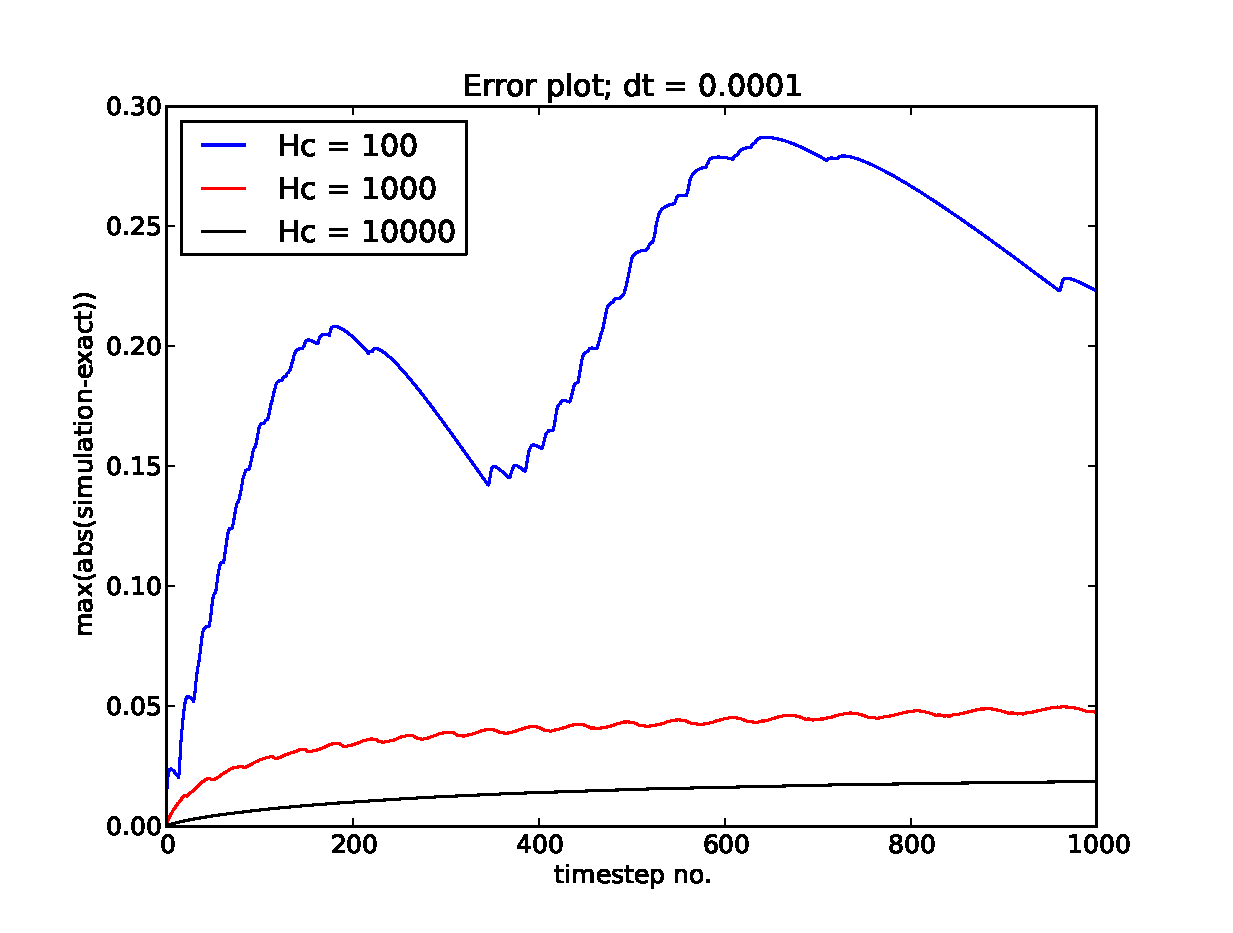
\includegraphics[width=\textwidth]{../doc/results/experiment_19112013_1625/results/errorplot.eps}
%  \caption{Using a normal $\Delta t = 0.0001$.}
%  \label{errorplot_BE1D_small_dt}
% \end{subfigure}
% \begin{subfigure}[b]{0.48\textwidth}
%  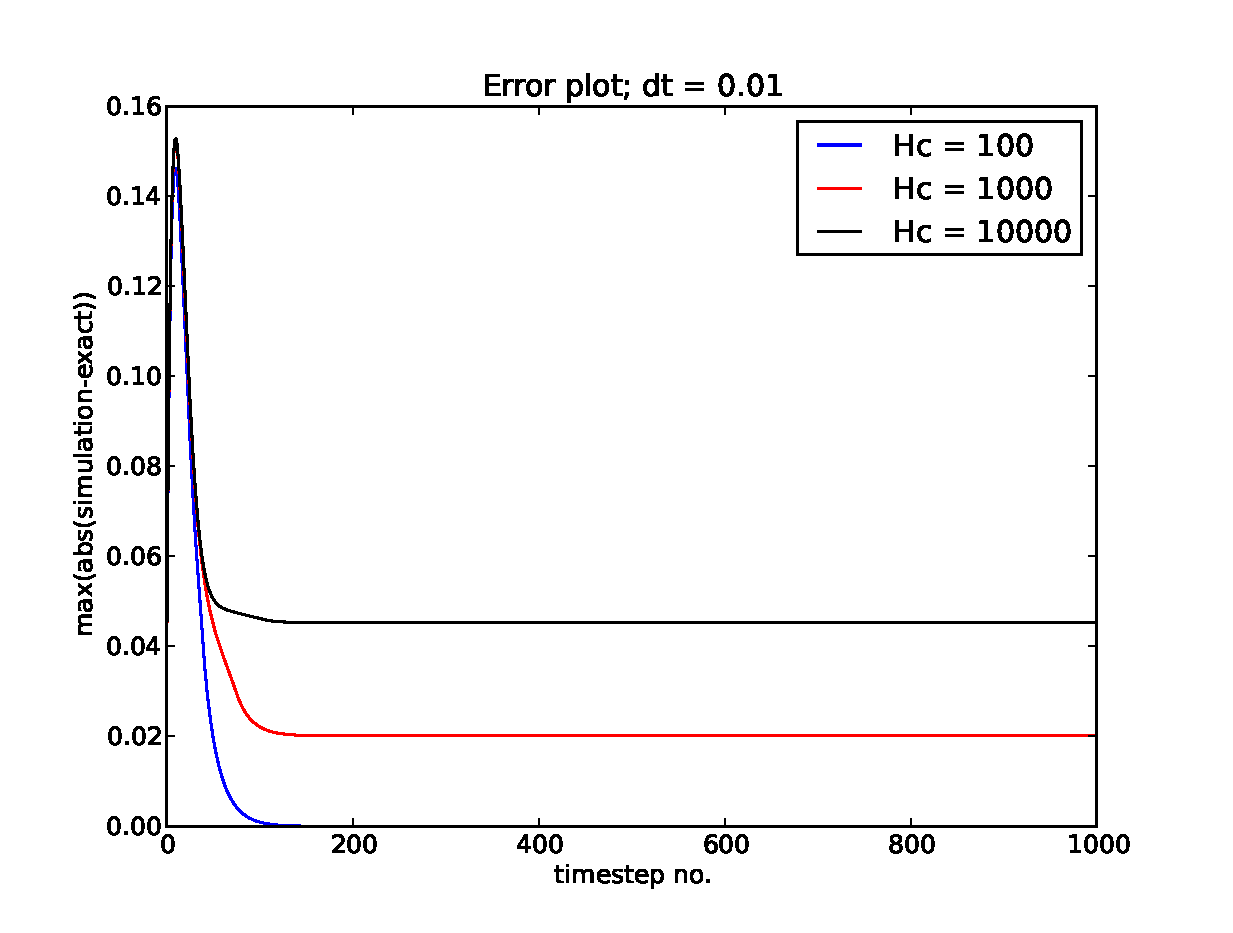
\includegraphics[width=\textwidth]{../doc/results/experiment_19112013_1627/results/errorplot.eps}
%  \caption{Using a large $\Delta t = 0.01$.}
%  \label{errorplot_BE1D_walk_large_dt}
% \end{subfigure}
% \caption{}
% \label{testing_dt_size}
% \end{figure}
% 
% \begin{figure}[H]
%  \centering
% \begin{subfigure}[b]{0.48\textwidth}
% 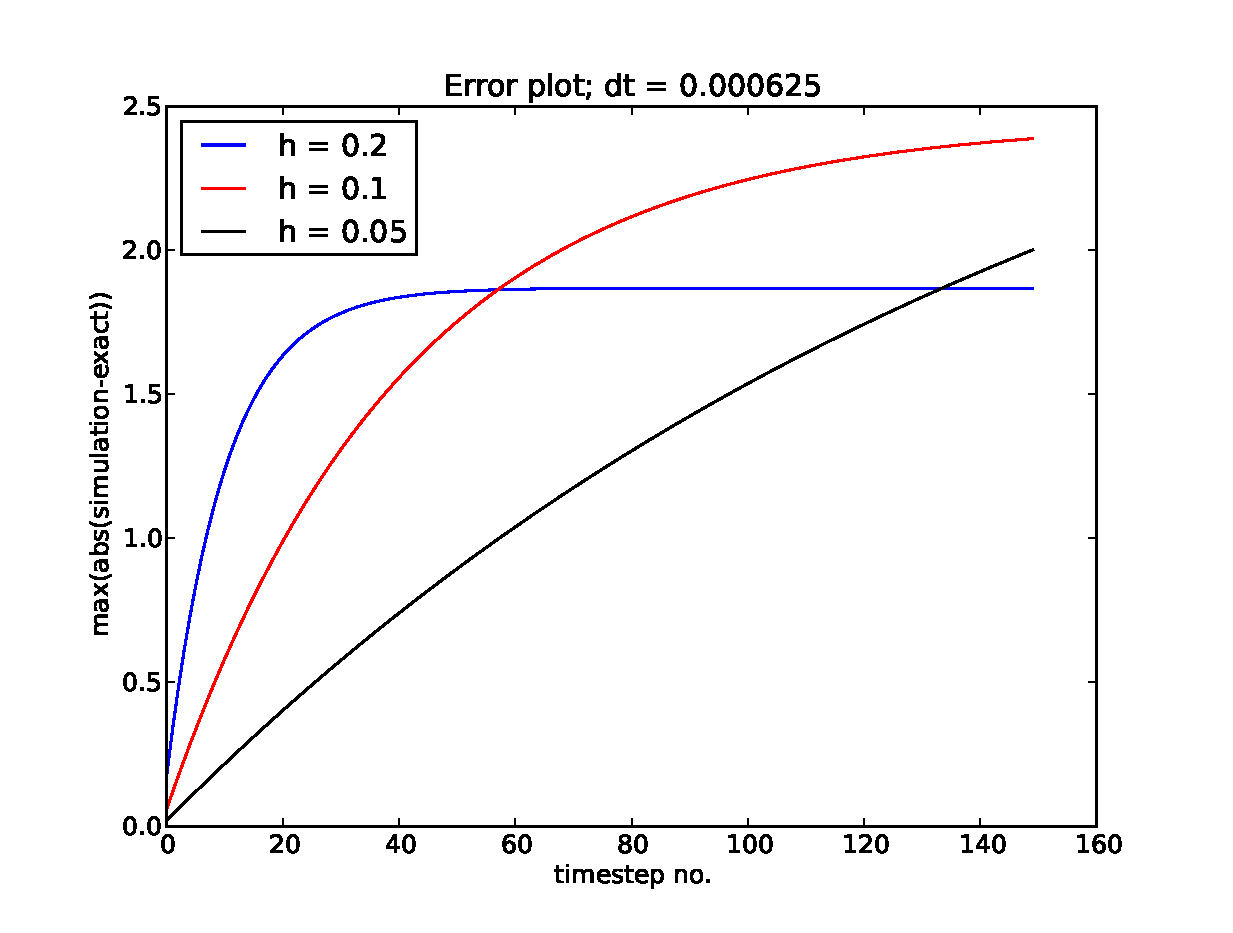
\includegraphics[width=\textwidth]{{../doc/results/experiment_02122013_1309_long_simulations_1d/results/errorplot}.eps}
%  \caption{}
%  \label{errorplot_FE_walk_long:normal}
% \end{subfigure}
% \begin{subfigure}[b]{0.48\textwidth}
%  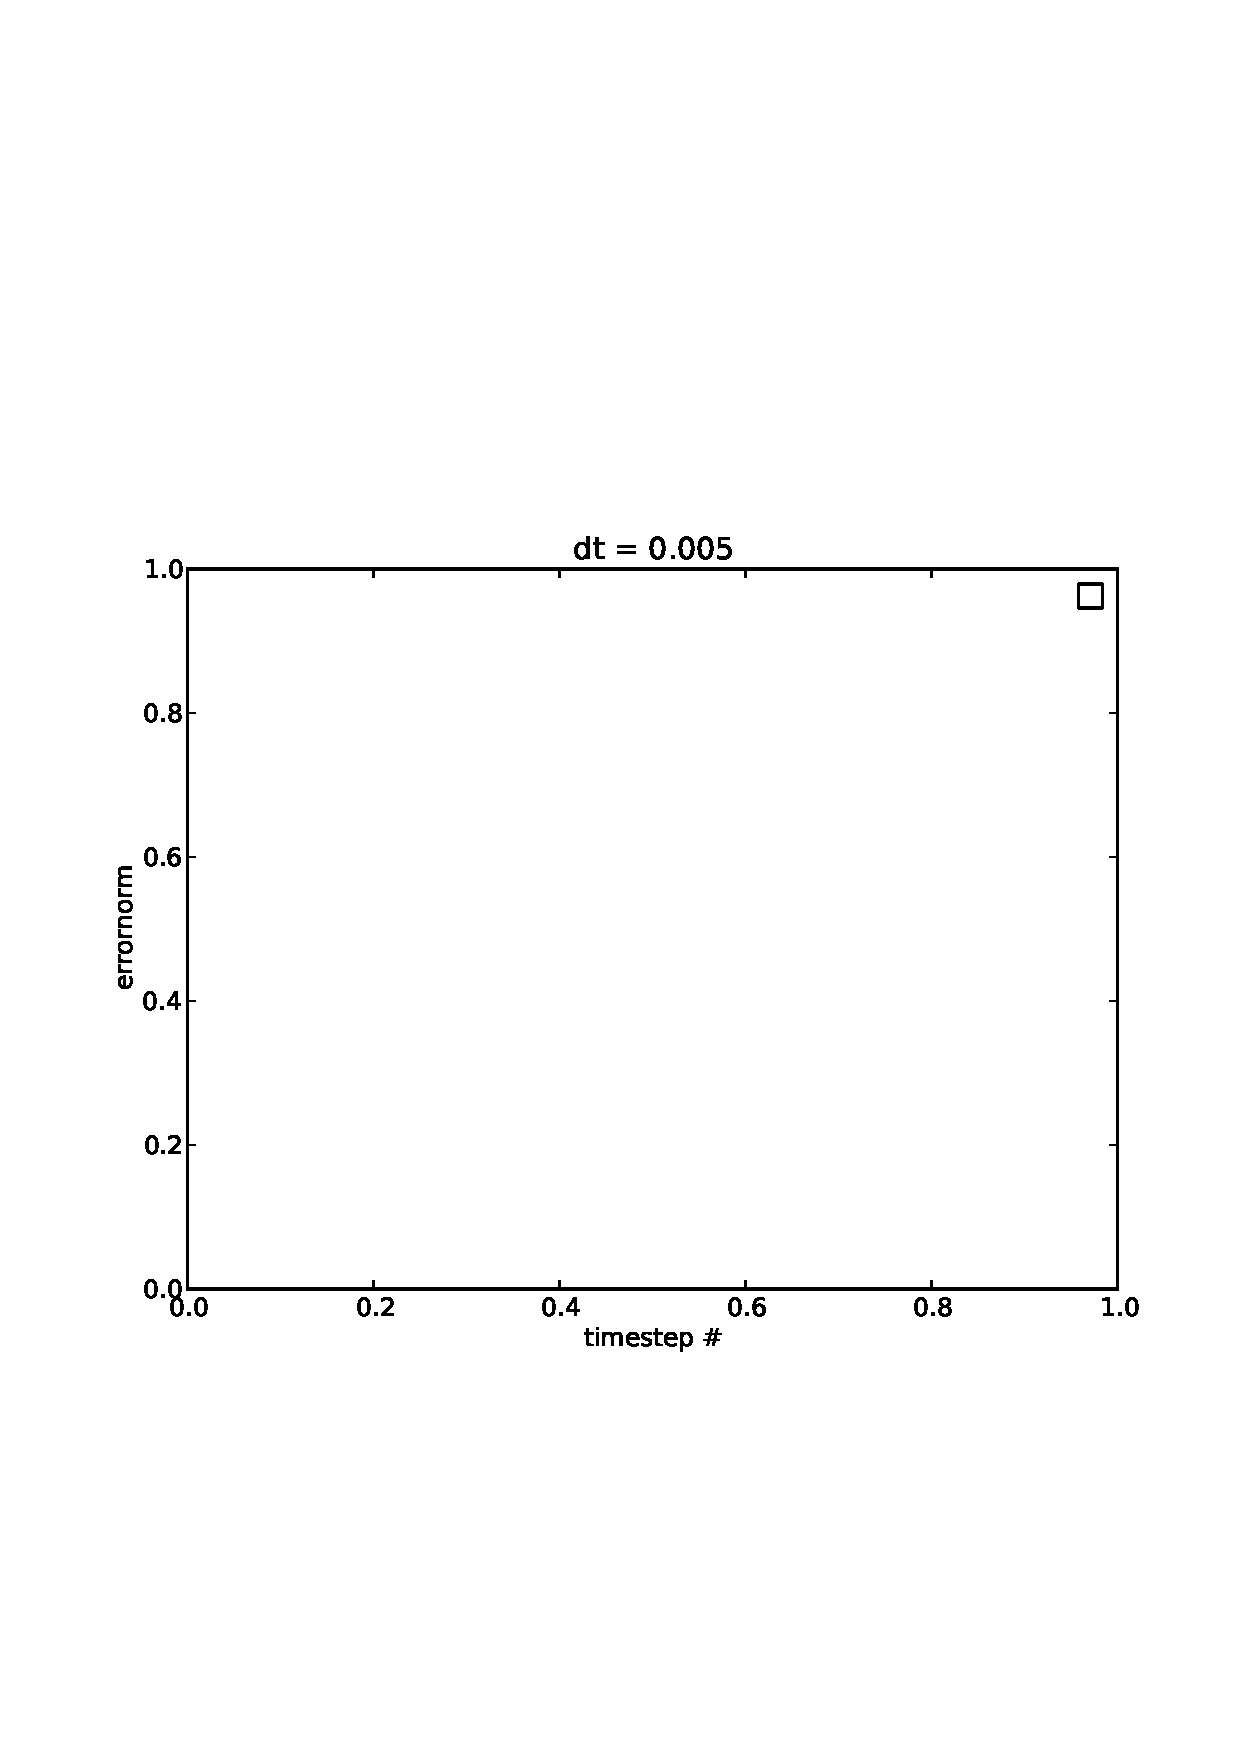
\includegraphics[width=\textwidth]{{../doc/results/experiment_02122013_1309_long_simulations_1d/results/deterministic_errorplot}.eps}
% \caption{}
% \label{errorplot_FE_walk_long:deterministic}
%  \end{subfigure}
% \caption[Error plot, long simulation]{The deterministic error and the error from simulations with walkers for long simulations.}
% \label{errorplot_FE_walk_long}
% \end{figure}
